\newif\ifisarxiv
\isarxivtrue


% ready for submission
% \ifisarxiv
%   \documentclass[11pt]{article}
%   \usepackage{fullpage}
% \else
%   \documentclass[twoside]{article}
%   \usepackage[accepted]{aistats2020}

%   % \special{papersize = 8.5in, 11in}
%   % \setlength{\pdfpageheight}{11in}
%   % \setlength{\pdfpagewidth}{8.5in}

%   \usepackage{natbib}
%   \renewcommand{\bibname}{References}
%   \renewcommand{\bibsection}{\subsubsection*{\bibname}}
% \fi
\documentclass[thesis.tex]{subfiles}



\begin{document}
\ifisarxiv
  \title{Bayesian experimental design using regularized \\
    determinantal point processes}
  \author{%
          Micha{\l } Derezi\'{n}ski \\
  Department of Statistics\\
  University of California, Berkeley\\
  \texttt{mderezin@berkeley.edu}\\
  \And
  Feynman Liang \\
  Department of Statistics\\
  University of California, Berkeley\\
  \texttt{feynman@berkeley.edu}
  \And
  Michael W. Mahoney\\
  ICSI and Department of Statistics\\
  University of California, Berkeley\\
  \texttt{mmahoney@stat.berkeley.edu}
    % examples of more authors
    % \And
    % Coauthor \\
    % Affiliation \\
    % Address \\
    % \texttt{email} \\
    % \AND
    % Coauthor \\
    % Affiliation \\
    % Address \\
    % \texttt{email} \\
    % \And
    % Coauthor \\
    % Affiliation \\
    % Address \\
    % \texttt{email} \\
    % \And
    % Coauthor \\
    % Affiliation \\
    % Address \\
    % \texttt{email} \\
  }
  \else
  
  \runningtitle{Bayesian experimental design using regularized DPPs}
  \twocolumn[
  \aistatstitle{Bayesian experimental design \\using regularized 
    determinantal point processes}
  \aistatsauthor{%
    Micha{\l } Derezi\'{n}ski
    \And
    Feynman Liang
    \And
    Michael W. Mahoney
  }
  \aistatsaddress {
    Department of Statistics\\
    University of California, Berkeley\\
    \texttt{mderezin@berkeley.edu}
    \And
    Department of Statistics\\
    University of California, Berkeley\\
    \texttt{feynman@berkeley.edu}
    \And
    ICSI and Department of Statistics\\
    University of California, Berkeley\\
    \texttt{mmahoney@stat.berkeley.edu}
  } 
% \aistatsauthor{ Author 1 \And Author 2 \And  Author 3 }
% \aistatsaddress{ Institution 1 \And  Institution 2 \And Institution 3 }
  ]
\fi

% The \author macro works with any number of authors. There are two commands
% used to separate the names and addresses of multiple authors: \And and \AND.
%
% Using \And between authors leaves it to LaTeX to determine where to break the
% lines. Using \AND forces a line break at that point. So, if LaTeX puts 3 of 4
% authors names on the first line, and the last on the second line, try using
% \AND instead of \And before the third author name.

% \ifisarxiv
%   \date{}
%   \def\And{\and}
% \fi

% \ifisarxiv
%   \maketitle
% \fi

% \begin{abstract}
We establish a fundamental connection between Bayesian
experimental design and determinantal point processes
(DPPs). Experimental design is a classical task in combinatorial
optimization, where we wish to select a small subset of $d$-dimensional
 vectors to minimize a statistical optimality criterion.
 We show that a new regularized variant of
 DPPs can be used to design
efficient algorithms for finding $(1+\epsilon)$-approximate solutions
to experimental design under four commonly used optimality
criteria: A-, C-, D- and V-optimality. A key novelty is that we offer
improved guarantees under the Bayesian framework.
Our algorithm returns a $(1+\epsilon)$-approximate solution when the
subset size $k$ is
$\Omega(\frac{d_{\A}}{\epsilon} + \frac{\log
1/\epsilon}{\epsilon^2})$, where $d_{\A}\ll d$ is an effective dimension
determined by prior knowledge (via a precision matrix $\A$). This is the first
approximation guarantee where the dependence on $d$ is
replaced by an effective dimension. Moreover, the time complexity
of our algorithm significantly improves on existing approaches
with comparable guarantees. 
% \end{abstract}


\section{Introduction}

Consider a collection of $n$ experiments parameterized by
$d$-dimensional vectors $\x_1,\dots,\x_n$, and let $\X$ denote the
$n\times d$ matrix with rows $\x_i^\top$. The outcome of the $i$th
experiment is a random variable $y_i = \x_i^\top\w + \xi_i$, where
$\w$ is the parameter vector of a linear model with prior distribution
$\Nc(\zero,\sigma^2\A^{-1})$, and $\xi_i\sim \Nc(0,\sigma^2)$ is
independent noise. In experimental design, we have access to the vectors 
$\x_i^\top$, for $i\in\{1,\ldots,n\} = [n]$, but we are allowed to
observe only a small number of outcomes $y_i$ for experiments we choose.
Suppose that we observe the outcomes from a subset
$S\subseteq [n]$ of $\lvert S \vert = k$ experiments. The
posterior distribution of $\w$ given $\y_S$ (the vector of outcomes in $S$) is:
\begin{align*}
  \w\mid \y_S \ &\sim\ \Nc(\mub, \Sigmab), \\
  \text{where } \mub &= (\X_S^\top\X_S + \A)^{-1}\X_S^\top\y_S, \\
  \Sigmab &= \sigma^2(\X_S^\top\X_S+\A)^{-1}.
\end{align*}
Here, $\X_S$ is the $k\times d$ matrix with rows $\x_i^\top$ for
$i\in S$.

In Bayesian experimental design \citep{bayesian-design-review},
the prior precision matrix $\A$ is used to encode prior knowledge
and our goal is to choose $S$ so as to 
  minimize a function (a.k.a.~an optimality criterion) measuring the ``size''
  of the posterior covariance matrix
  $\Sigmab_{\w\mid\y_S} = \sigma^2(\X_S^\top\X_S+\A)^{-1}$.
Note that $\Sigmab_{\w\mid\y_S}$ is well defined even if $\A$ is not
invertible (i.e., an ``improper prior''). In particular, it includes classical
experimental design as the special case $\A = \zero$, as well as
the ridge-regularized case for $\A=\lambda\I$.
Denoting $\Sigmab$ as the subset covariance $\X_S^\top\X_S$, we will
use $f_{\A}(\Sigmab)$ to represent the following standard Bayesian 
optimality criteria \citep{bayesian-design-review,optimal-design-pukelsheim}:
\begin{enumerate}
\item A-optimality:\quad $f_{\A}(\Sigmab) = \tr\big((\Sigmab+\A)^{-1}\big)$;
\item C-optimality:\quad \!\!$f_{\A}(\Sigmab) = \cb^\top(\Sigmab+\A)^{-1}\cb$ for
$\cb \in \R^d$;
\item D-optimality:\quad $f_{\A}(\Sigmab) = \det(\Sigmab+\A)^{-1/d}$;
  \item V-optimality:\quad $f_{\A}(\Sigmab) =
    \frac1n\tr\big(\X(\Sigmab+\A)^{-1}\X^\top\big)$.
  \end{enumerate}
  Applications including clinical trials
  \citep{ryan2015fully,ding2008bayesian,spiegelhalter2004incorporating,berry2002adaptive,stangl1998bayesian,flournoy1993clinical},
  medical imaging \citep{owen2016optimisation},
  materials science
  \citep{frazier2016bayesian,ueno2016combo,terejanu2012bayesian},
 and biological process models \citep{ryan2016optimal}
  all use these optimality criteria and thus stand to benefit from
  our contributions.
  % Our algorithm can also be directly applied to improve
  % approximate design methods which leverage normal-based approximations
  % \citep{overstall2018approach}.

The general task we consider is the following combinatorial
optimization problem, where $[n]$
denotes $\{1,...,n\}$:

%\noindent
\textbf{Bayesian experimental design.}
Given an $n\times d$ matrix $\X$,
a criterion $f_{\A}(\cdot)$ and~$k\in[n]$,
efficiently compute or approximate
\begin{align*}
\argmin_{S \subseteq [n]} f_{\A}(\X_S^\top\X_S)\quad\text{subject
  to}\quad |S|=k.
\end{align*}
We denote the value at the optimal solution as $\opt$.
The prior work around this problem can be grouped into two research questions.
% categories, each asking a question about the optimum of the above
% problem, which we will denote $\opt =
% \min_{S:|S|=k}f_{\A}(\X_S^\top\X_S)$.
The first question asks when does there exist a
polynomial time algorithm for finding a $(1+\epsilon$)-approximation
for $\opt$.
The second question asks what we can
infer about $\opt$ just from the spectral
information about the problem, which is contained in the
data covariance matrix~$\Sigmab_\X=\X^\top\X$.

% We aim to address two research questions which have been outlined
% by the prior work on this topic:
%\noindent

\textbf{Question 1:} \quad
Given $\X$, $f_{\A}$ and $k$, can we efficiently find a $(1+\epsilon)$-approximation for
$\opt$?

\textbf{Question 2:} \quad
Given only $\Sigmab_{\X}$, $f_{\A}$ and $k$,
what is the upper bound on $\opt$?


A key aspect of both of these questions is how large the subset
size $k$ has to be for us to provide useful answers. As a baseline, we
should expect meaningful results when $k$ is at least $\Omega(d)$ \citep[see
discussion in][]{near-optimal-design}, and in fact,
for classical experimental design (i.e., when $\A=\zero$), the problem
becomes ill-defined 
when $k<d$. In the Bayesian setting we should be able to exploit the
additional prior knowledge 
to achieve strong results even for $k\ll d$. Intuitively, the larger
the prior precision matrix $\A$, the fewer degrees of freedom we have
in the problem. To measure this, we use the statistical notion of
\emph{effective dimension} \citep{ridge-leverage-scores}.
\begin{definition}
For $d\times d$ positive semi-definite (psd) matrices $\A$ and $\Sigmab$,
  let the $\A$-effective dimension of $\Sigmab$
be defined as $d_{\A}(\Sigmab) =
\tr\big(\Sigmab(\Sigmab+\A)^{-1}\big) \leq d$.
We will use the shorthand $d_{\A}$ when referring to $d_{\A}(\Sigmab_{\X})$.
\end{definition}
\cite{klivans-goel17} showed that $d_\A$ can be orders of
  magnitude smaller than the 
actual dimension $d$ when the eigenvalues of $\Sigmab_\X$ exhibit fast
decay, which is often the case in real datasets
\citep{revisiting-nystrom}. Recently,
\cite{regularized-volume-sampling} obtained bounds on Bayesian 
A/V-optimality criteria for $k\geq d_{\A}$, suggesting that $d_{\A}$
is the right notion of degrees of freedom for this problem.

\subsection{Main results}
Our main results provide new answers to Questions 1 and 2
by proposing a novel algorithm for Bayesian experimental design with
strong theoretical guarantees.

  \paragraph{Answer to Question 1.}
We propose an efficient $(1+\epsilon)$-approximation algorithm for
A/C/D/V-optimal Bayesian  experimental design:
\begin{theorem}\label{t:q2}
  Let $f_{\A}$ be A/C/D/V-optimality and $\X$ be $n\times d$. If
  $k=\Omega\big(\frac{d_{\A}}{\epsilon} +
  \frac{\log1/\epsilon}{\epsilon^2}\big)$ for some $\epsilon\in(0,1)$, then 
we can find in polynomial time a subset $S$ of size $k$ s.t.
  \begin{align*}
    f_{\A}\big(\X_S^\top\X_S\big) \leq (1+\epsilon)\cdot\opt.
  \end{align*}
\end{theorem}
\begin{remark}
  The algorithm referred to in Theorem~\ref{t:q2} first solves a convex
  relaxation of the task via a semi-definite program (SDP) to find a
  weight vector $p\in[0,1]^n$, then uses our new randomized algorithm 
  to round the weights to $\{0,1\}$, obtaining the subset
  $S$. The expected cost after SDP is $O(ndk+k^2d^2)$.
\end{remark}
% Note that, unlike in Theorem \ref{t:q1}, we use the unrescaled effective
% dimension instead of the rescaled one, $d_{\frac nk\!\A}$. The
% actual effective dimension that applies here (given in the proof in
% Section \ref{s:guarantees}) depends on the SDP solution. It is
% always upper bounded by $d_{\A}$, but it may be significantly
% smaller.

A number of recent works studied $(1+\epsilon)$-approximate SDP-based algorithms 
for classical and Bayesian experimental design (see Table
\ref{tab:comp} and Section \ref{s:related-work} for a comparison). Unlike \emph{all} prior work on
this topic, we are able to eliminate the
dependence of the subset size $k$ on the dimension $d$, replacing it
with the potentially much smaller effective dimension $d_\A$.
Our result also improves over the existing approaches in terms of the computational
cost of the rounding procedure that is performed after solving the SDP. A
number of different methods can be used to solve the SDP relaxation (see
Section \ref{s:experiments}). For
example, \cite{near-optimal-design} suggest using an iterative
optimizer called entropic mirror descent, which is known to exhibit
fast convergence and can run in $O(nd^2T)$ time, where $T$ is the
number of iterations. 

\begin{figure*}[htbp]
  \centering
\begin{tabular}{r||c|c|l|l}
  &Criteria&Bayesian& $k$ %& dep.~on $d$ & dep.~on $1/\epsilon$
  & Cost after SDP\\%of rounding\\
  \hline\hline
\small  \cite{tractable-experimental-design}
  &\small A,V&\xmark  &$d^2/\epsilon$
  % &\Red{quadratic}& \Orange{linear}
  &$n^2\cdot d$\\
\small  \cite{near-optimal-design}
  &\small A,C,D,E,G,V&\cmark
&$ d/\epsilon^2$
% &\Orange{linear}& \Red{quadratic}
  &$n\cdot kd^2$\\ 
\small  \cite{proportional-volume-sampling}
  &\small A,D&\xmark &$d/\epsilon$
  % & \Orange{linear}& \Orange{linear}
  & $n^4\cdot k^2d$\\ 
  \hline
  \small\textbf{this paper}&\small A,C,D,V&\cmark
    & $d_{\A}/\epsilon$
    % &\Green{none}& \Orange{linear}
  & $n\cdot kd + k^2d^2$
\end{tabular}
\captionof{table}{Comparison of SDP-based $(1+\epsilon)$-approximation algorithms for
  classical and Bayesian experimental design (X-mark means that only
  the classical setting applies).
In the cost analysis, $n$ could be replaced by the number of
non-zero weights in the SDP solution. For simplicity we omit the log
terms and assume that $\epsilon = \Omega(\frac1{d_{\A}})$. Our
approach beats other methods both in terms of the
runtime and the dependence of $k$ on $d$ (when $d_\A=o(d)$).} 
\label{tab:comp}
\end{figure*}


\paragraph{Answer to Question 2.}
%Formalizing the above intuitions,
By performing a careful theoretical analysis of the performance of our
algorithm, we are able to give an improved upper bound on $\opt$. In the below
result, we use a more refined notion of effective dimensionality for
Bayesian experimental design,
$d_{\frac nk\A}$ (where the precision matrix $\A$ is scaled by factor $\frac
nk$), which is smaller than $d_\A$ and therefore leads 
to a tighter bound.
% $d_{\frac nk\A}\leq d_{\A}$ as the notion of 
% effective dimensionality, which is an improvement over the prior work
% We now present our first main result, which provides an analytic bound
% on the four optimality criteria listed above (Question 1) for most
% practically relevant values of $k$.
\begin{theorem}\label{t:q1}
  Let $f_{\A}$ be A/C/D/V-optimality and $\X$ be
  $n\times d$. For any $k$ such that $k\geq 4d_{\frac
    nk\!\A}$, %we have
  \begin{align*}
\opt    \leq \bigg(\ 1+8\,\frac{d_{\frac
    nk\!\A}}{k} + 8\sqrtshort{\frac{\ln (k/d_{\frac nk\!\A})}{k}}\
    \bigg)\cdot f_{\A}\big(\tfrac kn\Sigmab_{\X}\big).
  \end{align*}
\end{theorem}
\begin{remark}
  We give a (randomized) algorithm which (with probability 1) finds
  the subset $S$ that certifies this bound and has expected time
  complexity $O(ndk+k^2d^2)$. 
  % and is $O(t (n d^2 + k d^2))$ time with
  % probability exponentially increasing in $t$.
  % Michal: please check this statement.
\end{remark}
  In particular, this means that if $k\geq 4d_{\frac nk\!\A}$
  then there is $S$ of size $k$
  which satisfies $f_{\A}(\X_S^\top\X_S) = O(1)\cdot f_{\A}(\frac kn\Sigmab_{\X})$.
  This not only improves on \cite{regularized-volume-sampling} in terms
  of the supported range of sizes $k$, but also in terms of the obtained bound (see
  Section \ref{s:related-work} for a~comparison). In Section
  \ref{s:experiments}, we we provide numerical evidence suggesting
  that for many real datasets the quantity $f_{\A}(\frac
  kn\Sigmab_{\X})$ provides a good estimate for $\opt$ to within a
  factor of 2.

Theorem \ref{t:q1} suggests that the right notion of degrees of
freedom for Bayesian experimental design can in fact be smaller
than $d_{\A}$.  
Intuitively, since $d_{\A}$ is computed using the full data covariance
$\Sigmab_{\X}$, it is not in the same scale as the smaller covariance
$\X_S^\top\X_S$ based on the subset $S$ of size $k\ll n$. In our
result this is corrected by increasing the 
regularization on $\Sigmab_\X$ from $\A$ to $\frac{n}{k}\A$ and using
$d_{\frac nk\A}=d_{\frac{n}{k}\A}(\Sigmab_\X)$ as the degrees of
freedom. 
Note that $d_{\frac nk\!\A}\leq d_{\A}$ and this gap can be very large for some
problems (see discussion in Appendix~\ref{a:deff}).





\subsection{Technical contributions}
  To establish Theorems \ref{t:q2} and \ref{t:q1}, 
  we develop a theoretical framework for a new sampling distribution
  % $\DPPreg{p}(\X,\A)$, where 
  % $p=(p_1,...,p_n)\in[0,1]^n$ is a vector of weights. 
  which can be seen as a \emph{regularized} variant of a determinantal point
  process (DPP). DPPs are a well-studied family of distributions
with numerous applications in sampling diverse subsets
  of negatively correlated elements \citep[see][]{dpp-ml}.

  Given a psd matrix $\A$ and a weight vector $p=(p_1,...,p_n)\in[0,1]^n$, we
define $\DPPreg{p}(\X,\A)$ as a distribution over subsets $S\subseteq[n]$ (of all
sizes) such that (see Definition~\ref{d:r-dpp}):
\begin{align*}
 \Pr(S)\propto \det(
  \X_S^\top\X_S+\A)\ \cdot \prod_{i\in S}p_{i}\cdot\prod_{i\not\in
  S}(1-p_i).
\end{align*}
A number of regularized DPPs have been proposed recently
\citep{dpp-intermediate,regularized-volume-sampling}, mostly within the context
of Randomized Numerical Linear Algebra (RandNLA)~
\citep{Mah-mat-rev_JRNL,DM16_CACM,RandNLA_PCMIchapter_TR}.
To our knowledge, ours is the first such definition that strictly falls
under the umbrella of traditional DPPs \citep{dpp-ml}.
We show this in Section \ref{s:r-dpp}, where we also prove that
regularized DPPs can be decomposed into a low-rank DPP plus
i.i.d. Bernoulli sampling (Theorem \ref{t:algorithm}). This decomposition reduces
the sampling cost from $O(n^3)$ to $O(nd^2)$,
and involves a more general result about DPPs defined via a
correlation kernel (Lemma~\ref{l:decomposition}), which is of
independent interest.

In Section \ref{s:guarantees} we demonstrate a fundamental connection between an
$\A$-regularized DPP and Bayesian experimental design with precision
matrix $\A$. For simplicity of exposition, let the weight vector $p$ be uniformly equal $(\frac kn,...,\frac kn)$. If
$S\sim\DPPreg{p}(\X,\A)$ and $f_{\A}$ is any one of the
A/C/D/V-optimality criteria, then:
 \begin{align*}
   \E\big[f_{\A}(\X_S^\top\X_S)\big]
   \leq f_{\A}\big(\tfrac kn\Sigmab_{\X}\big)
   \quad\text{and}\quad \E\big[|S|\big]
   \leq d_{\frac nk\!\A}+k. 
 \end{align*}
The proof of Theorem \ref{t:q1} relies on these two inequalities and a
concentration bound for the subset size $|S|$,
whereas to obtain Theorem
\ref{t:q2} we additionally use the SDP relaxation to find the optimal
weight vector~$p$. When $\A=\zero$, then $\DPPreg{p}(\X,\A)$ bears a
lot of similarity to 
\emph{proportional volume sampling} which is an (unregularized) determinantal
distribution proposed by \cite{proportional-volume-sampling}.
Our algorithm not only extends it to the Bayesian setting but also
offers a drastic time complexity improvement from 
the $O(n^4dk^2\log k)$ required by \cite{proportional-volume-sampling}
down to the $O(nd^2)$ required for sampling from $\DPPreg{p}(\X,\A)$,
and recent advances in RandNLA for DPP sampling
\citep{leveraged-volume-sampling,correcting-bias,dpp-intermediate} suggest that
$O(nd\log n + \poly(d))$ time is also possible.





\section{Related work}
\label{s:related-work}

A number of works proposed $(1+\epsilon)$-approximation algorithms
for experimental design which start with solving a convex
relaxation of the problem, and then use some rounding strategy to
obtain a discrete solution (see Table \ref{tab:comp} for comparison).
In this line of work we wish to find the smallest $k$ for which a
polynomial time approximation algorithm is possible. For example,
\cite{tractable-experimental-design} gave an approximation algorithm
for classical A/V-optimality with $k=\Omega(\frac{d^2}{\epsilon})$, where the
rounding is done in a greedy fashion, and some randomized rounding
strategies are also discussed. \cite{proportional-volume-sampling}
suggested \emph{proportional volume sampling} for the rounding step
and obtained approximation algorithms for classical A/D-optimality with
$k=\Omega(\frac d\epsilon+\frac {\log1/\epsilon}{\epsilon^2})$. Their
approach is particularly similar to ours (when $\A=\zero$). However,
as discussed earlier, while their algorithms run in polynomial time,
they scale very poorly with the number of experiments $n$ (see Table 
\ref{tab:comp}). \cite{near-optimal-design} proposed  
an efficient algorithm with a $(1+\epsilon)$-approximation guarantee for a wide
range of optimality criteria, including A/C/D/E/V/G-optimality, both classical and Bayesian, when
$k=\Omega(\frac d{\epsilon^2})$.  Our results (in Theorem \ref{t:q2}) improve on this work in
two important ways: 
\begin{itemize}
  \item In terms of the dependence on $\epsilon$ for A/C/D/V-optimality,
  \item In terms of the dependence on the dimension 
  (by replacing $d$ with $d_{\A}$) in the Bayesian setting.
\end{itemize}
A lower bound shown by \cite{proportional-volume-sampling} implies that our
Theorem \ref{t:q2} cannot be
directly extended to E-optimality, but a similar lower bound does not
exist for G-optimality. We remark that the approximation approaches
relying on a convex relaxation can generally be converted to
an upper bound on $\opt$ akin to our Theorem \ref{t:q1},
however, unlike our bound, none of them apply to the regime of $k\leq d$.


Non-trivial bounds for the \emph{classical} A-optimality criterion
(i.e., $\opt$
with $\A=\zero$) were first given by \cite{avron-boutsidis13}, where
they show that
for any $k\geq d$, $\opt \leq (1+ \frac{d-1}{k-d+1})\cdot f_{\zero}(\frac kn\Sigmab_\X)$
and the subset $S$ attaining the bound can be found in polynomial time.
The result was later extended \citep{unbiased-estimates,
regularized-volume-sampling,unbiased-estimates-journal} to the case
where $\A=\lambda\I$, proving that for any $k\geq d_{\lambda\I}$,
we have
$\opt\leq (1 +\frac{d_{\lambda\I}-1}{k-d_{\lambda\I}+1})\cdot f_{\frac
  kn\!\lambda\I}(\frac kn\Sigmab_\X)$,
and also a faster $O(nd^2)$ time algorithm was provided.
In comparison, our results (in Theorem \ref{t:q1}) offer the following
improvements for upper bounding $\opt$:
\begin{itemize}
  \item We cover a wider range of subset sizes, because
    $d_{\frac nk\!\lambda\I}\leq d_{\lambda\I}$,
  \item Our upper bound can be much tighter because
    $f_{\lambda\I}(\frac kn\Sigmab_\X)\leq f_{\frac kn\!\lambda\I}(\frac
    kn\Sigmab_\X)$. 
\end{itemize}
Additionally, \cite{minimax-experimental-design} propose a new notion of
\emph{minimax} experimental design, which is related to A/V-optimality.  They
also use a determinantal distribution for subset selection, however, due to
different assumptions, their bounds are incomparable.

Purely greedy approximation algorithms have been shown to provide
guarantees in a number of special cases for experimental design. One
example is classical D-optimality criterion, which can be converted to
a submodular function \citep{submodularity-optimal-design}. Also, greedy algorithms
for Bayesian A/V-optimality criteria have been considered by
\cite{greedy-supermodular} and \cite{greedy-graph-sampling}. These
methods can only provide a constant factor approximation guarantee
(as opposed to $1+\epsilon$), and the factor is generally problem
dependent (which means it could be arbitrarily large).
Finally, a number of
heuristics with good empirical performance have been proposed, such as Fedorov's
exchange method \citep{cook1980comparison}. However, in this work
we focus on methods that provide theoretical approximation guarantees.
% In Section \ref{s:experiments} we experimentally show that
% our regularized DPP sampling (without solving an SDP) performs
% better than iid sampling methods like uniform and predictive length
% sampling \cite{zhu2015optimal} and that by using the SDP solution
% we can improve it to match the performance of
% greedy algorithms for A-optimal design \cite{chamon2017approximate,greedy-supermodular}
% which empirically have been found to perform well on real world data.


\section{A new regularized determinantal point process}
\label{s:r-dpp}
  In this section we develop the theory for a novel regularized extension of
  determinantal point processes (DPP) which we use as the sampling distribution
  for obtaining guarantees in Bayesian experimental design.
  DPPs form a family of distributions which are used to model repulsion between
  elements in a random set, with many applications in machine learning
  \citep{dpp-ml}. Here, we focus on the setting where we are sampling out of all
  $2^n$ subsets $S\subseteq[n]$. Traditionally, a DPP is defined by a
  correlation kernel, which is an $n\times n$ psd matrix $\K$ with eigenvalues
  between 0 and 1, i.e., such that $\zero\preceq\K\preceq \I$. Given a
  correlation kernel $\K$, the corresponding DPP is
  defined as
  \begin{align*}
    S\sim\DPPcor(\K)\quad\text{iff}\quad
    \Pr(T\subseteq S) = \det(\K_{T,T})\ \  \forall_{T\in[n]},
  \end{align*}
where $\K_{T,T}$ is the submatrix of $\K$ with rows and columns
indexed by $T$. Another way of defining a DPP, popular in the machine
learning community, is via an ensemble kernel $\L$. Any psd matrix
$\L$ is an ensemble kernel of a DPP defined as:
  \begin{align*}
    S\sim\DPPens(\L)\quad\text{iff}\quad \Pr(S) \propto \det(\L_{S,S}).\quad~
  \end{align*}
Crucially, every $\DPPens$ is also a $\DPPcor$, but not the other way
around. Specifically, $\DPPens(\L)=\DPPcor(\K)$ when:
\begin{align*}
  &\text{(a)}\ \  \L=\K(\I-\K)^{-1},\qquad
  &\text{(b)}\ \  \K = \I -  (\I+\L)^{-1},
\end{align*}
but (a) requires that $\I-\K$ be invertible which is not true
for some DPPs.
(This will be important in our analysis.)
The classical algorithm for sampling from a DPP requires the
eigendecomposition of either matrix $\K$ or $\L$, which in general
costs $O(n^3)$, followed by a sampling procedure which costs
$O(n\,|S|^2)$ \cite{dpp-independence,dpp-ml}.

We now define our regularized DPP and describe its
connection with correlation and ensemble~DPPs.
\begin{definition}\label{d:r-dpp}
Given matrix $\X\in\R^{n\times d}$, a sequence  $p=(p_1,\dots,p_n)\in[0,1]^n$
and a psd matrix $\A\in\R^{d\times d}$ such that
$\sum_ip_i\x_i\x_i^\top\!+\A$ is
full rank, let
$\DPPreg{p}(\X,\A)$ be a distribution over $S\subseteq [n]$:
  \begin{align}
  \Pr(S) = \frac{\det(
  \X_S^\top\X_S+\A)}{\det\!\big(\!
 \sum_ip_i\x_i\x_i^\top\!+ \A\big)}
\cdot \!\prod_{i\in S}p_{i}\cdot\!\prod_{i\not\in S}(1\!-\!p_i).\label{eq:poisson-prob}
\end{align}
%   \Pr(\pi)\ \propto\ \det\!\big(\A +
%   \X_{\pi}^\top\X_{\pi}\big)
%   \Pr\!\bigg(\Big[K\!=\!|\pi|\Big]\,\wedge\,\Big[\forall_{i=1}^{|\pi|}\,\pi_i\!=\!\pi_i\Big] \bigg).
% \end{align*}
\end{definition}
The fact that this is a proper distribution (i.e., that it sums to
one) can be restated as a determinantal expectation formula: if
$b_i\sim\mathrm{Bernoulli}(p_i)$ are independent Bernoulli random
variables, then
\begin{align*}
  &\sum_{S\subseteq [n]}\!\det(
  \X_S^\top\X_S+\A)\prod_{i\in S}p_{i}\prod_{i\not\in S}(1-p_i) \\
  &\!=
  \E\bigg[\!\det\!\Big(\sum_ib_i\x_i\x_i^\top\!+\A\Big)\bigg]\overset{(*)}{=}
  \det\!\Big(\sum_i\E[b_i]\x_i\x_i^\top\!+\A\Big),
\end{align*}
where $(*)$ follows  from Lemma 7 of \citet{determinantal-averaging}.
% follows from a recently shown determinantal expectation formula.
% \begin{lemma}[\cite{determinantal-averaging}]\label{l:cb}
% For $\X\!\in\!\R^{n\times d}$, $\A\!\in\!\R^{d\times d}$
% and a random set $S\subseteq [n]$ drawn with independent Bernoullis,
% \begin{align*}
%   \E\Big[\det\!\big(\X_S^\top\X_S+\A\big)\Big]
%   = \det\!\Big( \E\big[\X_S^\top\X_S\big]+\A\Big).
% \end{align*}
% \end{lemma}

  The main theoretical contribution in this section is the
  following efficient algorithm for $\DPPreg{p}(\X,\A)$ which reduces it to
  sampling from a correlation DPP and unioning with i.i.d.~Bernoulli samples:
\begin{theorem}\label{t:algorithm}
For any $\X\in\R^{n\times d}$, $p\in[0,1]^n$ and a psd matrix $\A$
s.t.~$\sum_ip_i\x_i\x_i^\top\!+\A$ is
full rank, let
\begin{align*}
  T&\sim\DPPcor\big(\D_p^{\sfrac12}\X(\A+\X^\top\D_p\X)^{-1}\X^\top\D_p^{\sfrac12}\big),
  \quad\\
  &\quad\text{where}\quad\D_p=\diag(p).
\end{align*}
If $b_i\sim\mathrm{Bernoulli}(p_i)$ are independent random variables, then
$T\cup \{i:b_i\!=\!1\}\sim \DPPreg{p}(\X,\A)$.
\end{theorem}

\begin{remark}
    Figure~\ref{fig:algorithm-pseudocode} illustrates how to exploit this result
    to build an efficient sampling algorithm.
  Since the correlation kernel matrix has rank at most $d$, the preprocessing
  cost of eigendecomposition is $O(nd^2)$. Then, each sample costs only $O(n\,|T|^2)$.
\end{remark}

We prove the theorem in three steps. 
First, we express $\DPPreg{p}(\X,\A)$ as an ensemble DPP, which requires some
additional assumptions on $\A$ and $p$ to be possible.
Then, we convert the ensemble to a correlation kernel (eliminating the extra
assumptions),
and finally show that this kernel can be decomposed into a rank $d$ kernel plus
Bernoulli sampling.
In the process, we establish several novel theoretical properties
regarding the representation, decomposition, and closure properties
of regularized DPPs which may be of independent interest.

\renewcommand{\thealgorithm}{}
\floatname{algorithm}{}
\vspace{-3mm}
\begin{figure}[htbp]
\begin{center}
  \begin{algorithm}[H]
    {\fontsize{9}{9}\selectfont
      \caption{\bf \small Sampling \ $S\sim\DPPreg{p}(\X,\A)$}
      \begin{algorithmic}[0]
        \STATE \textbf{Input:} $\X\!\in\!\R^{n\times d}\!,\text{ psd } \A\!\in\!\R^{d\times
        d}\!, p\!\in\![0,1]^n$\\[1mm]
        \STATE Compute $\Z \leftarrow \A+\X^\top\D_p\X$\\[1mm]
        \STATE Compute \textsc{SVD} of  $\B=\D_p^{\sfrac12}\X\Z^{-\sfrac12}$\\[1mm]
        \STATE Sample $T\sim\DPPcor(\B\B^\top)$ \hfill \citep{dpp-independence}\\[1mm]
        \STATE Sample $b_i\sim\mathrm{Bernoulli}(p_i)$ for $i\in[n]$\\[1mm]
        \RETURN $S=T\cup\{i:b_i=1\}$
      \end{algorithmic}
    }
  \end{algorithm}
\end{center}
\vspace{-3mm}
\caption{Algorithm which exploits
  Theorem~\ref{t:algorithm} to sample $S \sim \DPPreg{p}(\X, \A)$
  in $O( nd^2 )$ time.}
\label{fig:algorithm-pseudocode}
\end{figure}


\vspace{2mm}
\begin{lemma}\label{t:reduction}
  Given $\X$, $\A$ and $\D_p$ as in Theorem \ref{t:algorithm}, assume that $\A$ and $\I-\D_p$ are
  invertible. Then,
  \begin{align*}
    \DPPreg{p}(\X,\A)&=\DPPens\big(\Dbt+
    \Dbt^{\sfrac12}\X\A^{-1}\X^\top
    \Dbt^{\sfrac12}\big),\quad\\
    \text{where}
    \quad\Dbt &= \D_p(\I-\D_p)^{-1}.
  \end{align*}
\end{lemma}
\begin{proof}
  Let $S\sim \DPPreg{p}(\X,\A)$. By Definition \ref{d:r-dpp} and
  the fact that $\det(\A\B+\I)=\det(\B\A+\I)$,
  \begin{align*}
    \Pr(S) &\propto \det(\X_S^\top\X_S+\A)\cdot
\prod_{i\in S}p_i\cdot\prod_{i\not\in S}(1-p_i) \\
&= \det(\X_S^\top\X_S+\A)\cdot
\prod_{i\in S}\frac{p_i}{1-p_i}\cdot\prod_{i=1}^n(1-p_i)
\\ &\propto\det\!\big(\A(\A^{-1}\X_S^\top\X_S+\I)\big) \det(\Dbt_{S,S}) \\
     &=\det(\A)\det(\A^{-1}\X_S^\top\X_S+\I) \det(\Dbt_{S,S})
\\ &\propto \det(\X_S \A^{-1}\X_S^\top+\I) \det(\Dbt_{S,S}) \\
&=\det\!\Big(\big[\Dbt^{\sfrac12}\X \A^{-1}\X^\top\Dbt^{\sfrac12}+\Dbt\big]_{S,S}\Big),
  \end{align*}
which matches the definition of the L-ensemble DPP.
\end{proof}
 At this point, to sample from  $\DPPreg{p}(\X,\A)$, we could simply
invoke any algorithm for sampling from
an ensemble DPP. However, this would only work for invertible
$\A$, which in particular excludes the important case of
$\A=\zero$ corresponding to classical experimental
design. Moreover, the standard algorithm would require computing the
eigendecomposition of the ensemble kernel, which (at
least if done na\"ively) costs $O(n^3)$. Even after this is done, the
sampling cost would still be $O(n\,|S|^2)$ which can be considerably
more than $O(nd^2)$. We first address the issue of invertibility of matrix
$\A$ by expressing our distribution via a correlation DPP.
\begin{lemma}\label{l:correlation}
  Given $\X$, $\A$, and $\D_p$ as in Theorem \ref{t:algorithm} (without
  any additional assumptions), we have
  \begin{align*}
    &\DPPreg{p}(\X,\A) 
    = \DPPcor\big(\D_p + \\
    &\ (\I\!-\!\D_p)^{\sfrac12}\,\D_p^{\sfrac12}\X(\A\!+\!\X^\top\D_p\X)^{-1}\X^\top\D_p^{\sfrac12}(\I\!-\!\D_p)^{\sfrac12}\big).
    \end{align*}
  \end{lemma}
  When $\A$ and $\I-\D_p$ are invertible, then the proof (given in
  Appendix \ref{a:proofs}) is a straightforward calculation.
Then, we use a limit argument with $p_\epsilon=(1-\epsilon)p$ and
$\A_\epsilon=\A+\epsilon\I$, where $\epsilon\rightarrow 0$.

Finally, we show that the correlation DPP arrived at in Lemma
\ref{l:correlation} can be decomposed into a smaller DPP plus
Bernoulli sampling. In fact, in the following lemma we obtain a more
general recipe for combining DPPs with Bernoulli sampling, which may
be of independent interest. Note that if $b_i\sim\mathrm{Bernoulli}(p_i)$ are independent random
variables then $\{i:b_i\!=1\!\}\sim\DPPcor(\D_p)$.
\begin{lemma}\label{l:decomposition}
  Let $\K$ and $\D$ be $n\times n$ psd matrices with eigenvalues between
0 and 1, and assume that $\D$ is diagonal. If\, $T\!\sim\DPPcor(\K)$ and
$R\sim\DPPcor(\D)$, then
\begin{align*}T\cup R\sim \DPPcor\big(\D+(\I-\D)^{\sfrac12}\K
  (\I-\D)^{\sfrac12}\big).
  \end{align*}
\end{lemma}
The lemma is proven in Appendix \ref{a:proofs}. Theorem
\ref{t:algorithm} now follows by combining Lemmas \ref{l:correlation} and \ref{l:decomposition}.

\section{Guarantees for Bayesian experimental design}
\label{s:guarantees}
In this section we prove our main results regarding Bayesian
experimental design (Theorems \ref{t:q2} and \ref{t:q1}). First, we
establish certain properties of the regularized DPP distribution that
make it effective in this setting. Even though the size of the
sampled subset $S\sim\DPPreg{p}(\X,\A)$ is random and can be as large
as $n$, it is also highly concentrated around its expectation, which
can be bounded in terms of the $\A$-effective dimension. This is
crucial, since both of our main results require a subset of
deterministically bounded size. Recall that the effective dimension is
defined as a function $d_{\A}(\Sigmab) =
\tr\big(\Sigmab(\A+\Sigmab)^{-1}\big)$. The omitted proofs are in
Appendix \ref{a:proofs}.
\begin{lemma}\label{l:size}
  Given any $\X\in\R^{n\times d}$, $p\in[0,1]^n$ and a psd matrix $\A$
s.t.~$\sum_ip_i\x_i\x_i^\top\!+\A$ is
full rank, let $S=T\cup \{i:b_i=1\}\sim \DPPreg{p}(\X,\A)$ be defined
as in Theorem \ref{t:algorithm}. Then
\begin{align*}
  \E\big[|S|\big] &\leq \E\big[|T|\big] + \E\Big[\sum_i b_i\Big]  \\
                  & = d_{\A}\Big(\sum_ip_i\x_i\x_i^\top\Big) + \sum_i p_i.
\end{align*}
\end{lemma}
Next, we show two expectation inequalities for the matrix inverse and
matrix determinant, which hold for the regularized DPP.
We use them to bound the Bayesian optimality criteria in expectation.
% These are
% immediately followed by a corollary applying them to bound
% Bayesian optimality criteria.
\begin{lemma}\label{t:expectations}
Whenever $S\sim \DPPreg{p}(\X,\A)$ is a well-defined distribution it holds that
\begin{align}
  \E\Big[\big(\X_S^\top\X_S+\A\big)^{-1}\Big]
  &\preceq \Big(\!
    \sum_ip_i\x_i\x_i^\top \!+\A \Big)^{-1}\!\!,\label{eq:sqinv}
  \\
\E\Big[\!\det\!\big(\X_S^\top\X_S+\A\big)^{-1}\Big]
  &\leq\det\!\Big(\!
    \sum_ip_i\x_i\x_i^\top\!+\A \Big)^{\!-1}\!\!.\!\!\label{eq:det}
\end{align}
\end{lemma}
\begin{corollary}\label{c:expectations}
Let $f_{\A}$ be A/C/D/V-optimality. Whenever $S\sim\DPPreg{p}(\X,\A)$ is
well-defined,
\begin{align*}
  \E\big[f_{\A}(\X_S^\top\X_S)\big] \leq f_{\A}\Big(\sum_i p_i\x_i\x_i^\top\Big).
\end{align*}
\end{corollary}
\begin{proof}
  In the case of A-, C-, and V-optimality, the function $f_{\A}$ is a
  linear transformation of the matrix $(\X_S^\top\X_S+\A)^{-1}$ so the
  bound follows from \eqref{eq:sqinv}. For D-optimality, we apply
  \eqref{eq:det} as follows:
  \begin{align*}
    \E\big[f_{\A}(\X_S^\top\X_S)\big]
    & = \E\Big[\det\!\big(\X_S^\top\X_S+\A\big)^{-\sfrac1d}\Big] \\
    &\leq
     \E\bigg[\Big(\det\!\big(\X_S^\top\X_S+\A\big)^{-\sfrac1d}\Big)^d\bigg]^{\sfrac1d} \\
    \\ &=  \E\Big[\!\det\!\big(\X_S^\top\X_S+\A\big)^{-1}\Big]^{\sfrac1d}\\
       &\leq
         \det\!\Big(\sum_i p_i\x_i\x_i^\top\Big)^{-\sfrac1d},
  \end{align*}
  which completes the proof.
\end{proof}
Finally, we present the key lemma that puts everything together. This
result is essentially a generalization of Theorem \ref{t:q1} from
which also follows Theorem \ref{t:q2}.
\begin{lemma}\label{l:guarantees}
  Let $f_{\A}$ be A/C/D/V-optimality and $\X$ be $n\times
  d$.  For some $w=(w_1,\dots,w_n)\in[0,1]^n$, let
  $\Sigmab_w=\sum_iw_i\x_i\x_i^\top$ and assume that
  $\sum_i w_i=k\in[n]$. If $k\geq 4\,d_{\A}(\Sigmab_w)$, then a
subset $S\subseteq[n]$ of size $k$ can be found in $O(ndk+k^2d^2)$ time that satisfies
  \begin{align*}
    &f_{\A}\big(\X_S^\top\X_S\big)  \\
    &\leq \bigg(\ 1+8\,\frac{d_{\A}(\Sigmab_w)}{k} + 8\sqrtshort{\frac{\ln (k/d_{\A}(\Sigmab_w))}{k}}\ \bigg)\cdot f_{\A}\big(\Sigmab_w\big).
  \end{align*}
  \end{lemma}
\begin{proof}
  Let $p=(p_1,\dots,p_n)$ be defined so that $p_i =
  \frac{w_i}{1+\epsilon}$, and suppose that $S\sim
  \DPPreg{p}(\X,\A)$. Then, using Corollary \ref{c:expectations}, we have
  \begin{align*}
\Pr&\big(|S|\leq k\big)\,\E\Big[f_{\A}(\X_S^\top\X_S)\mid |S|\leq k\Big]\\
&\leq
\E\big[f_{\A}(\X_S^\top\X_S)\big] \\
&\leq
f_{\A}\Big(\sum_ip_i\x_i\x_i^\top\Big)
\\ &\leq (1+\epsilon)\cdot f_{\A}\Big(\sum_iw_i\x_i\x_i^\top\Big).
  \end{align*}
  Using Lemma \ref{l:size} we can bound the expected size of $S$ as
follows:
\begin{align*}
  \E\big[|S|\big]
  &\leq d_{\A}(\Sigmab_w) + \sum_i p_i \\
  &=d_{\A}(\Sigmab_w)+\frac{k}{1+\epsilon}\\
  &=k\cdot \Big(1+\frac {d_{\A}(\Sigmab_w) }k - \frac{\epsilon}{1+\epsilon}\Big).
\end{align*}
Let $d_w = d_{\A}(\Sigmab_w)$ and $\alpha=1+\frac {d_w} k -\frac{\epsilon}{1+\epsilon}$.
If $1\geq\epsilon\geq \frac{4d_w}{k}$, then $\alpha\leq 1 +
\frac\epsilon4-\frac\epsilon2=1-\frac\epsilon4$. Since $\DPPreg{p}(\X,\A)$
is a  determinantal point process, $|S|$ is a
Poisson binomial r.v.~so for $\epsilon\geq 6\sqrt{\frac{\ln(k/d_w)}{k}}$,
\begin{align*}
  \Pr(|S|>k) \leq \ee^{-\frac{(k-\alpha k)^2}{2k}} = \ee^{-\frac
  k2(1-\alpha)^2}\leq \ee^{-\frac{k\epsilon^2}{32}}\leq \frac{d_w}k.
\end{align*}
% If $k\geq\frac{4 d_{\A}(\Sigmab_w)}\epsilon$,
% then $\alpha \leq 1 + \frac\epsilon4 -\frac\epsilon2=1-\frac\epsilon4$.
%  Since $\Vol_p(\X,\A)$ is a determinantal point process, Lemma
% \ref{l:concent} implies that for $\epsilon'=\frac\epsilon4$ and $k\geq
%  48\frac{\ln 1/\epsilon'}{\epsilon'^2}$ we have
% \begin{align*}
% \Pr(|S|> k)\leq  \Pr\big(|S|\ \geq\ \alpha k + \epsilon' k\big)\leq
%   3\ee^{-\frac{\epsilon'^2k^2}{16(\epsilon'k+2\alpha k)}} \leq
%   3\ee^{-\frac{\epsilon'^2k}{48}}\leq 3\epsilon'.
% \end{align*}
For any $\epsilon\geq
4\,\frac{d_w}k + 6\sqrt{\frac{\ln(k/d_w)}{k}}$, we have
\begin{align*}
\E&\big[f_{\A}(\X_S^\top\X_S)\mid |S|\leq k\big] \\
&\leq \frac{1+\epsilon}{1-\frac{d_w}k}\cdot f_{\A}(\Sigmab_w)\\
  &\leq
  \bigg(1+\frac{\epsilon+\frac{d_w}k}{1-\frac{d_w}k}\bigg)\cdot
f_{\A}(\Sigmab_w)
\\ &\leq \bigg(1+7\,\frac{d_w}{k} +
  8\sqrtshort{\frac{\ln(k/d_w)}{k}}\bigg)\cdot f_{\A}(\Sigmab_w).
\end{align*}
Denoting $\E\big[f_{\A}(\X_S^\top\X_S)\mid |S|\leq k\big]$ as $F_k$,
Markov's inequality implies that
\[\Pr\Big(f_{\A}(\X_S^\top\X_S) \geq
  (1+\delta) F_k\ \mid\ |S|\leq k\Big)\leq \frac1{1+\delta}.\]
Also, we showed
that $\Pr(|S|\leq k)\geq 1-\frac{d_w}{k}\geq \frac34$. Setting $\delta=\frac{d_w}{C
  k}$ for sufficiently large $C$ we obtain that with probability
$\Omega(\frac{d_w}{k})$, the random set $S$ has size at most $k$ and
\begin{align*}
f_{\A}&(\X_S^\top\X_S) \\
&\leq \bigg(1+\frac{d_w}{C k}\bigg)\!\cdot\! \bigg(1+7\,\frac{d_w}{k} +
  8\sqrtshort{\frac{\ln(k/d_w)}{k}}\bigg)\!\cdot\! f_{\A}(\Sigmab_w)\\
&\leq
\bigg(1+8\,\frac{d_w}{k} +
  8\sqrtshort{\frac{\ln(k/d_w)}{k}}\bigg)\cdot f_{\A}(\Sigmab_w).
\end{align*}
We can sample from $\DPPreg{p}(\X,\A)$ conditioned on
$|S|\leq k$ and $f_{\A}(\X_S^\top\X_S)$ bounded as above by rejection
sampling. When $|S|<k$,  the set is completed to
$k$ with arbitrary indices. On average, $O(\frac k{d_w})$ samples from
$\DPPreg{p}(\X,\A)$ are needed, so the cost is $O(nd^2)$ for the
eigendecomposition, $O(\frac{k}{d_w}\cdot nd_w^2)=O(nd_wk)$ for
sampling and $O(\frac k{d_w}\cdot kd^2)$ for recomputing $f_{\A}(\X_S^\top\X_S)$.
\end{proof}
To prove the main results, we use Lemma \ref{l:guarantees} with
appropriately chosen weights $w$.
\begin{proofof}{Theorem}{\ref{t:q2}}
  As discussed by \cite{near-optimal-design} and
  \cite{boyd2004convex}, the following convex 
relaxation of experimental design can be written as a semi-definite
program and solved using standard SDP solvers:
\begin{align}
  &w^* \ = \  \argmin_w\ \
  f_{\A}\Big(\sum_{i=1}^nw_i\x_i\x_i^\top\Big),\quad\\
  &\text{subject to}\quad
  \forall_i\ \ 0\leq w_i\leq 1,\quad \sum_i w_i=k.\label{eq:sdp}
\end{align}
The solution $w^*$ satisfies $f_{\A}\big(\Sigmab_{w^*}\big)\leq
\opt$. If we use $w^*$ in Lemma \ref{l:guarantees}, then observing
that $d_{\A}(\Sigmab_{w^*})\leq d_{\A}$, and setting $k\geq C(\frac
{d_{\A}}{\epsilon} + \frac{\log1/\epsilon}{\epsilon^2})$ for
sufficiently large $C$, the algorithm in the lemma finds subset $S$
such that
\[f_{\A}(\X_S^\top\X_S)\leq (1+\epsilon)\cdot
f_{\A}(\Sigmab_{w^*})\leq
(1+\epsilon)\cdot\opt.\]
% \cite{tractable-experimental-design} show that
% the support of $w^*$ has size at most $k+d^2$, which reduces the cost of
% our sampling to $O(k^2d^2)$.
Note that we did not need to
solve the SDP exactly, so approximate solvers could be used instead.
\end{proofof}
\begin{proofof}{Theorem}{\ref{t:q1}}
Let $w=(\frac kn,...,\frac kn)$ in Lemma~\ref{l:guarantees}. Then, we have
$\Sigmab_w=\frac kn\Sigmab_{\X}$ and also $d_{\A}(\Sigmab_w) =
d_{\frac nk\!\A}$. Since for any set $S$ of size $k$, we
have $\opt\leq f_{\A}(\X_S^\top\X_S)$, the result follows.
\end{proofof}

\begin{figure*}
    \centering
    \hspace{-0.35cm}
    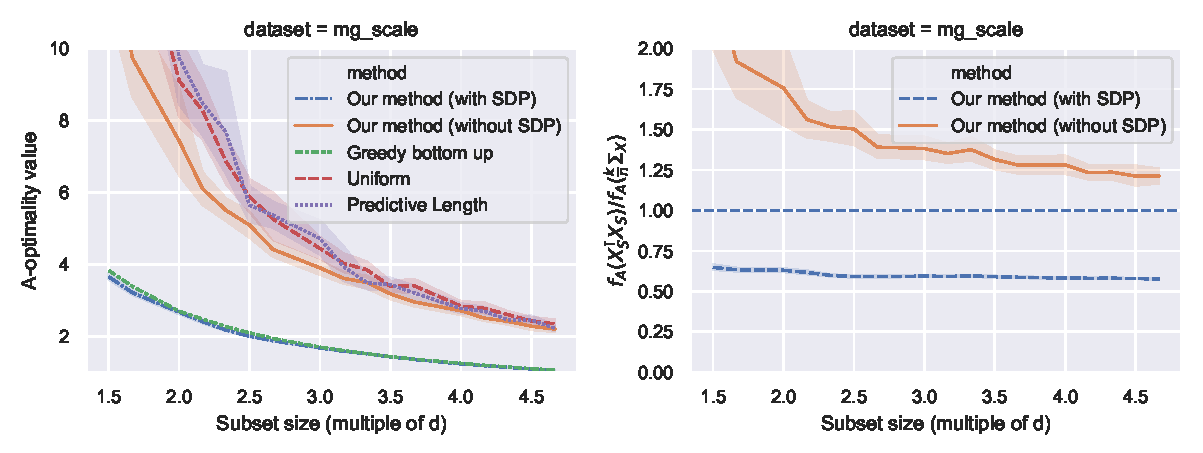
\includegraphics[width=\textwidth]{Figures/mg_combined.pdf}
    % 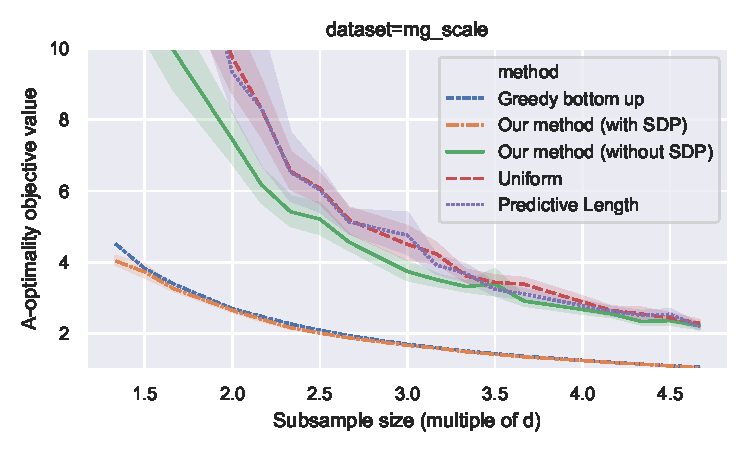
\includegraphics[width=0.51\textwidth]{bayesian_figures/objectives-mg_scale-full.pdf}\hspace{-2mm}\nobreak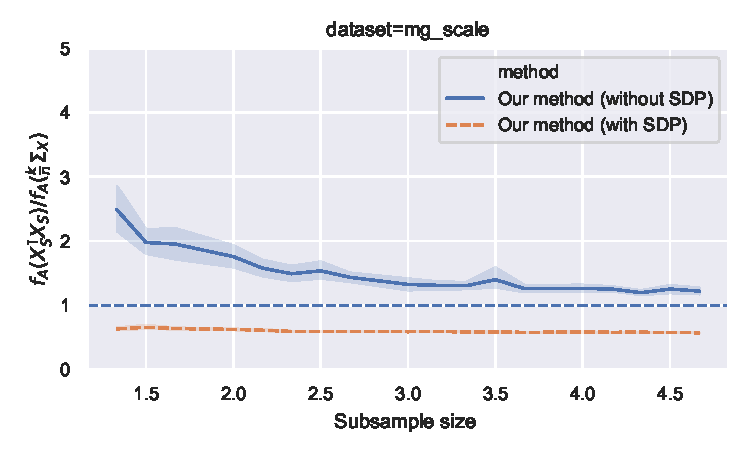
\includegraphics[width=0.51\linewidth]{bayesian_figures/ratios-mg_scale.pdf}
    % 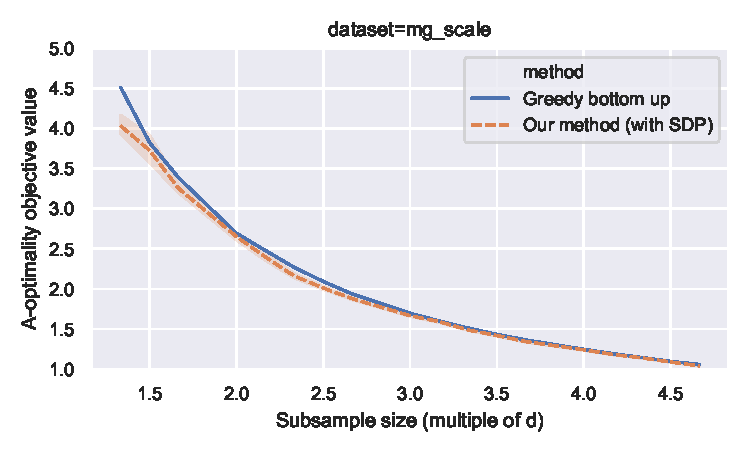
\includegraphics[width=0.49\textwidth]{bayesian_figures/objectives-mg_scale-zoom.pdf}
    \caption{(left) A-optimality value obtained by the various methods on
        the \texttt{mg\_scale} dataset \citep{libsvm} with
        prior precision $\A = 10^{-5}\, \I$,\quad (right)
        A-optimality value for our method (with and without SDP) divided by
        $f_{\A}(\frac kn\Sigmab_{\X})$, the baseline estimate suggested by Theorem \ref{t:q1}.}
    \label{f:experiments}
\end{figure*}

\section{Experiments}\label{s:bayesian:experiments}
We confirm our theoreticala
results with experiments on real world data from \texttt{libsvm} datasets
\citep{libsvm} (more details in Appendix~\ref{a:experiments}).
For all our experiments, the prior precision matrix is set to $\A = n^{-1} \I$
and we consider sample sizes $k \in [d, 5d]$. Each experiment is
averaged over 25 trials and bootstrap 95\% confidence intervals are shown.
% We provide open source implementations for efficient RDPP sampling
% and reproducing our results at \Red{TODO: fill in after blind review}.
The quality of our method, as measured by the A-optimality
criterion,
\[f_{\A}(\X_S^\top \X_S) = \tr \left((\X_S^\top \X_S + \A)^{-1}\right),\]
is compared against several baselines and recently proposed methods
for A-optimal design that have been shown to perform well in
practice. Note that none of these algorithms come with theoretical
guarantees as strong as those offered by our approach. The list of
implemented methods is as follows:
\begin{description}
    \item[Our method (with SDP)] uses the efficient algorithms
        developed in proving Theorem~\ref{t:q2} to sample
        $\DPPreg{p}(\X,\A)$ constrained to subset size $k$
        with $p = w^*$, see \eqref{eq:sdp},
        obtained using a         recently developed first order convex cone solver called Splitting
        Conical Solver \citep[SCS, see][]{o2016conic}.
        We chose SCS because it can handle the SDP constraints in
        \eqref{eq:sdp} and has provable termination guarantees, while
        also finding solutions faster \citep{o2016conic} than alternative
        off-the-shelf optimization software libraries such as SDPT3
        and Sedumi.

    \item[Our method (without SDP)] samples $\DPPreg{p}(\X,\A)$ with uniform
        probabilities $p \equiv \frac{k}{n}$.
        % Compared to uniform and predictive length
        %   sampling, there is an additional DPP sampling overhead which is independent
        %   of sample size $k$ (but does depend on $d$).

    \item[Greedy bottom-up] adds an index $i \in [n]$ to the sample $S$
        maximizing the increase in A-optimality criterion
        \citep{greedy-supermodular,chamon2017approximate}.
        %  This method posesses well-understood theoretical bounds
        %  (however they
        % require additional assumptions on the matrix $\X$) and has strong
        %  empirical performance \cite{tractable-experimental-design}.

    \item[Uniform] samples every size $k$ subset $S \subseteq [n]$
        with equal probability.

    \item[Predictive length] sampling \citep{zhu2015optimal} samples
        each row $\x_i$ of $\X$ with probability $\propto\|\x_i\|$.
\end{description}


Figure~\ref{f:experiments} reveals that our method (without SDP) is superior
to both uniform and predictive length sampling, producing designs which
achieve lower $A$-optimality criteria values for all sample sizes.
As Theorem~\ref{t:algorithm} shows that our method (without SDP) only differs
from uniform sampling by an additional DPP sample with controlled
expected size (see Lemma~\ref{l:size}), we may conclude
that adding even a small DPP sample can improve a uniformly sampled design.

Consistent with prior observations
\citep{tractable-experimental-design,chamon2017approximate}, the greedy bottom up
method achieves surprisingly good performance, despite the limited
theoretical guarantees it offers. However, if our method is used
in conjunction with an SDP solution, then we are able to match and
even slightly exceed the performance of the greedy bottom up
method. Furthermore, the overall run-time costs (see Appendix~\ref{a:experiments})
between the two are comparable. As the majority of the runtime of our
method (with SDP) is occupied by solving the SDP, an interesting future direction
is to investigate alternative solvers such as interior point methods as well
as terminating the solvers early once an approximate solution is reached.

Figure~\ref{f:experiments} (right) numerically evaluates the tightness of the
bound obtained in Theorem \ref{t:q1} by plotting the ratio:
\[\frac{f_{\A}(\X_S^\top \X_S)}{ f_{\A}(\frac{k}{n}\Sigmab_\X)}\]
for subsets returned by our method (with and without SDP). Note that the
line for our method with SDP on
Figure~\ref{f:experiments} (right) shows that the ratio never goes
below 0.5, and we saw similar behavior across all examined datasets
(see Appendix~\ref{a:experiments}). This evidence suggests that for
many real datasets $\opt$ is within only a small constant factor
away from $f_{\A}(\frac{k}{n}\Sigmab_\X)$, matching the upper bound of
Theorem~\ref{t:q1}.
% As sample size $k \to n$, this should converge towards $1$ because $\X_S^\top
% \X_S \to \X^\top \X = \Sigma_X$.
% Across all datasets we examined, we see that this ratio is close to
% its asymptotic value of $1$. Similar to how condition
% numbers are the proper problem dependent constants in matrix inversion
% \cite{nocedal2006numerical}
% and $\tr (\frac{k}{n} \X^\top \X)^{-1}$
% is the problem-dependent constant which appear in results on non-Bayesian
% experimental design \feynman{Citation for this COLT paper?}, our results here
% suggest that $f_{\A}\left(\frac{k}{n} \X^\top \X\right)$
% is the proper problem-dependent constant for Bayesian optimal experimental
% design with a $k$ cardinality constraint.
% \feynman{Does this make sense?}


% \section{Additional details for the experiments}
% \label{a:experiments}
\section*{Additional Experiments}

This section presents additional details and experimental results omitted from
the main body of the paper. In addition to the \texttt{mg\_scale} dataset presented in
Section~\ref{s:experiments}, we also benchmarked on three other data sets
described in Table~\ref{tab:libsvm-datasets}.
\begin{table}[ht]
    \centering
    \caption{\cite{libsvm} datasets used in experiments}
    \label{tab:libsvm-datasets}
    \begin{tabular}[t]{lcccc}
        \toprule
        & \texttt{mg\_scale} & \texttt{bodyfat\_scale} & \texttt{mpg\_scale} & \texttt{housing\_scale} \\
        \midrule
        $n$ & 1385 & 252 & 392 & 506 \\
        $d$ & 6 & 14 & 7 & 13\\
        \bottomrule
    \end{tabular}
\end{table}

The A-optimality values obtained are illustrated in Figure~\ref{f:obj-grid}.
The general trend observed in Section~\ref{s:experiments} of our method
(without SDP) outperforming independent sampling methods (uniform and
predictive length) and our method (with SDP) matching the performance of the
greedy bottom up method continues to hold across the additional datasets considered.

\begin{figure}[htpb]
    \centering
    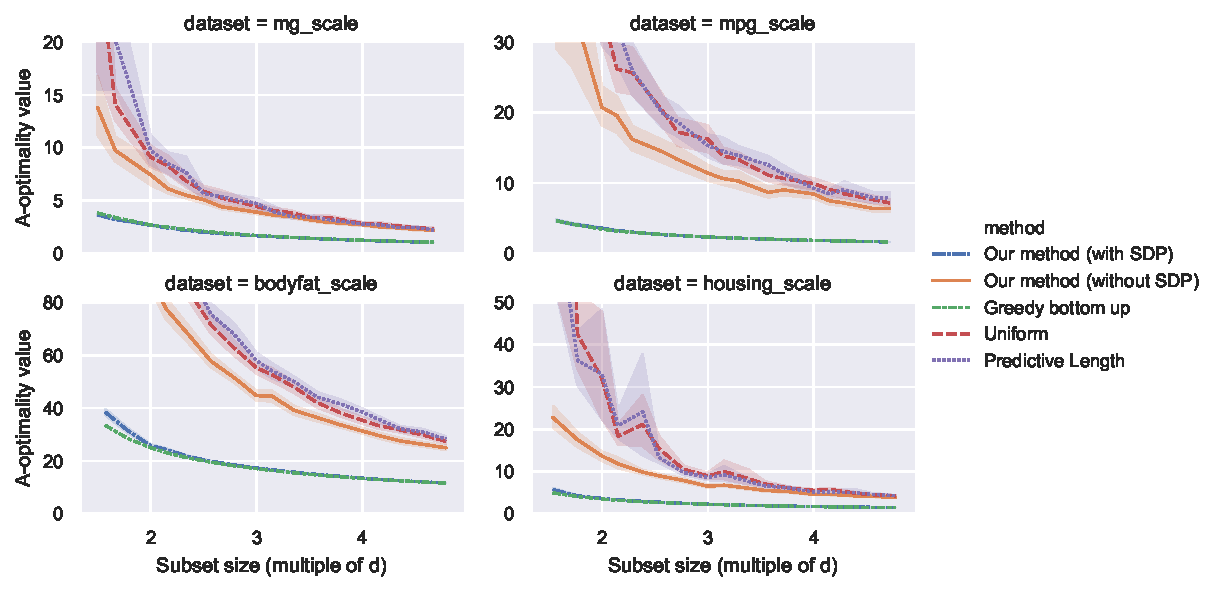
\includegraphics[width=\textwidth]{bayesian_figures/obj_grid.pdf}
    \caption{A-optimality values achieved by the methods compared. In all cases
        considered, we found our method (without SDP) to be superior to independent
        sampling methods like uniform and predictive length sampling. After paying the price
        to solve an SDP, our method (with SDP) is able to consistently match the performance
        of a greedy method which has been noted
        \cite{chamon2017approximate} to work well empirically.}
    \label{f:obj-grid}
\end{figure}

The relative ranking and overall order of magnitude differences
between runtimes (Figure~\ref{f:runtimes}) are also similar across the various
datasets. An exception to the rule is on $\texttt{mg\_scale}$, where we see
that our method (without SDP) costs more than the greedy method
(whereas everywhere else it costs~less).

\begin{figure}[htpb]
    \centering
    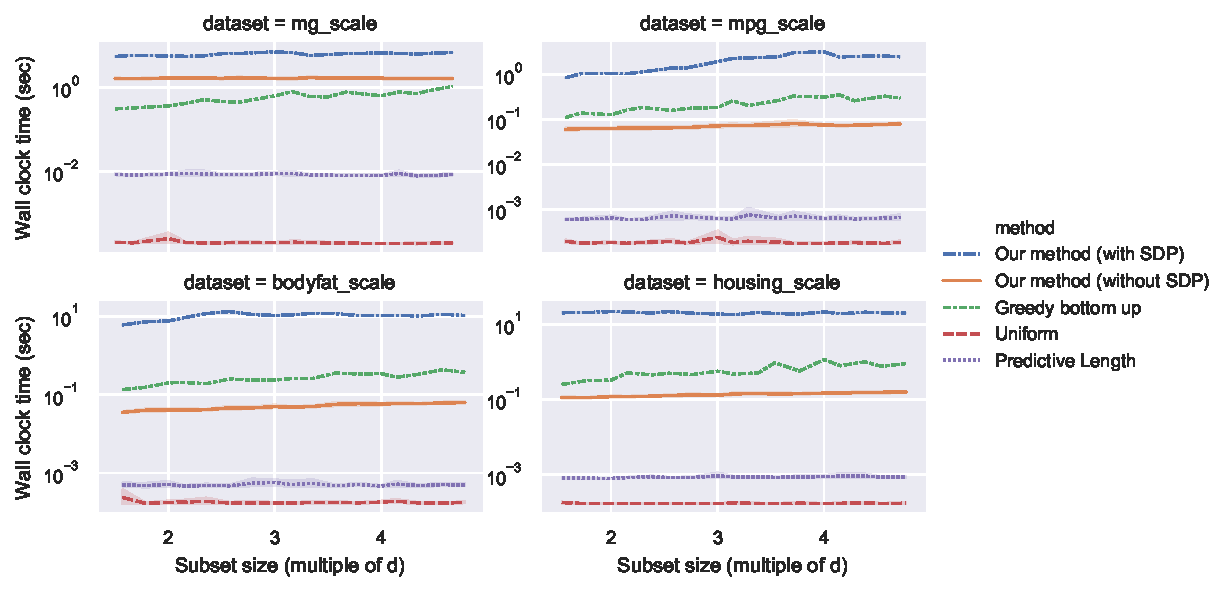
\includegraphics[width=\textwidth]{bayesian_figures/runtime_grid.pdf}
    \caption{Runtimes of the methods compared. Our method (without SDP) is
        within an order of magnitude of greedy bottom up and faster in 3 out of
        4 cases. The gap between our method with and without SDP is
        attributable to the SDP solver, making investigation of more efficient
        solvers and approximate solutions an interesting direction for future
        work.
    }
    \label{f:runtimes}
\end{figure}

The claim that $f_{\A}(\frac{k}{n} \Sigmab_\X)$ is an appropriate
quantity to summarize the contribution of problem-dependent factors
on the performance of Bayesian A-optimal designs is further evidenced in Figure~\ref{f:ratios}.
Here, we see that after normalizing the A-optimality values by this
quantity, the remaining quantities are all on the same scale and close to $1$.

\begin{figure}[htpb]
    \centering
    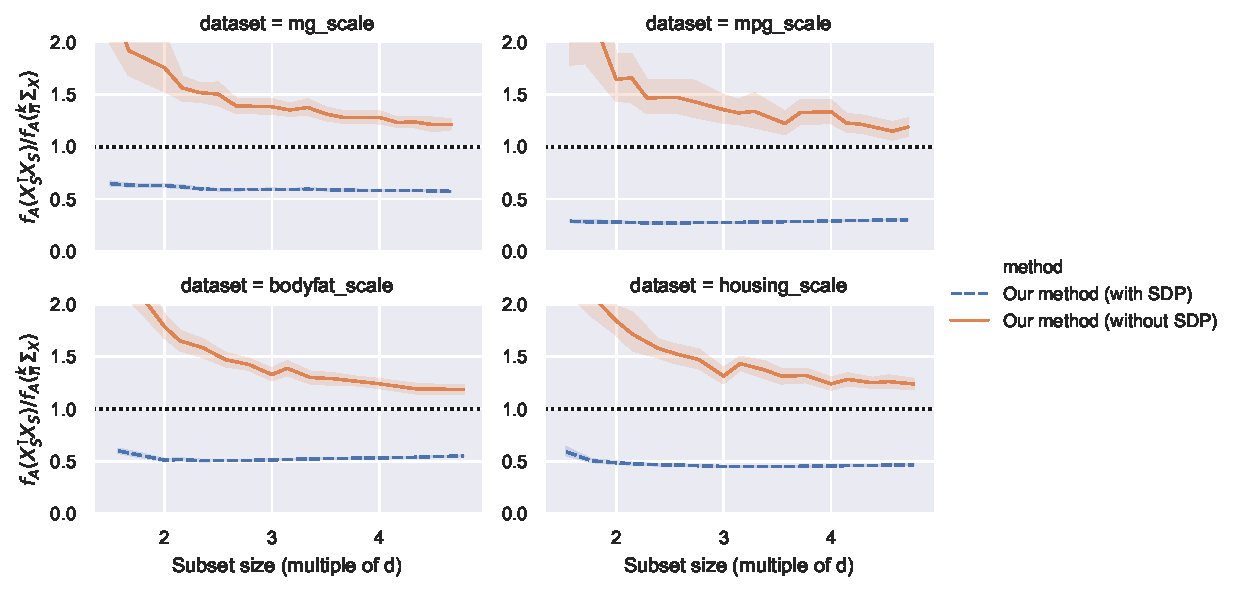
\includegraphics[width=\textwidth]{bayesian_figures/ratios_grid.pdf}
    \caption{The ratio controlled by Lemma~\ref{l:guarantees}. This ratio converges
        to $1$ as $k \to n$ and is close to $1$ across all
        real world datasets,
        suggesting that $f_{\A}(\frac{k}{n} \Sigmab_\X)$
        is an appropriate problem-dependent scale for Bayesian A-optimal
        experimental design.
    }
    \label{f:ratios}
\end{figure}

% The choice of $\lambda=43$ is motivated by keeping 95\% of the spectral
% mass. Figure~\ref{fig:scree} shows a scree plot for \texttt{mpg\_scale}
% after applying a polynomial kernel, where we see that the majority
% of the spectral mass is contained in the top few eigenvalues.

% \begin{figure}[htbp]
%     \centering
%     % \hspace{-0.55cm}
%     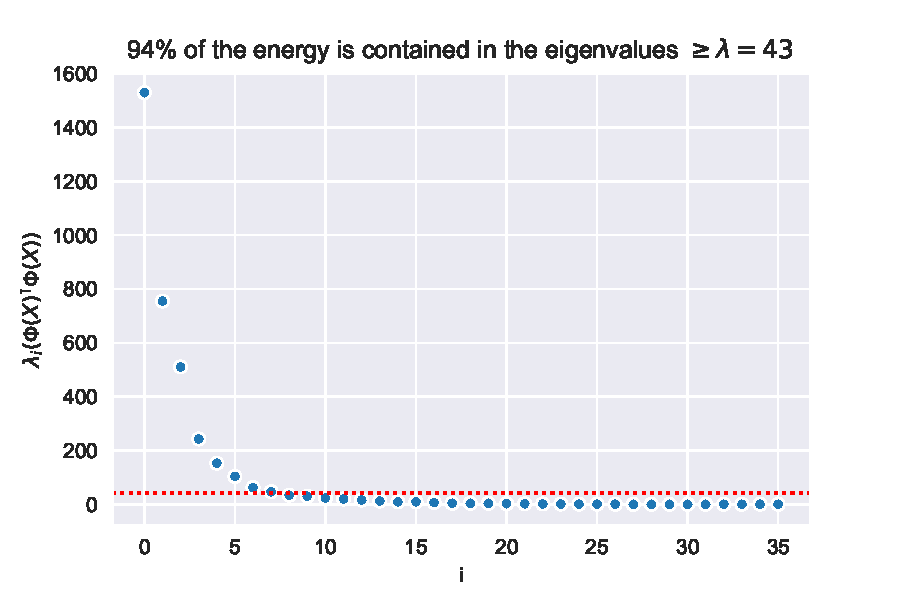
\includegraphics[width=0.5\textwidth]{Figures/screeplot.pdf}
%     \caption{
%         To determine the amount of regularization $\lambda$, a scree
%         plot of the eigenvalues of the polynomially expanded
%         covariance matrix $\Phi(X)^\top \Phi(X)$.
%     }
%     \label{fig:scree}
% \end{figure}

In addition to \texttt{mg\_scale}, the results for the low effective dimension
($d_\lambda$) ridge regression experiments on the remaining \texttt{libsvm}
datasets are shown in Figure~\ref{f:small_deff_ridge_and_a_opt}.

\begin{figure}[htpb]
    \centering
    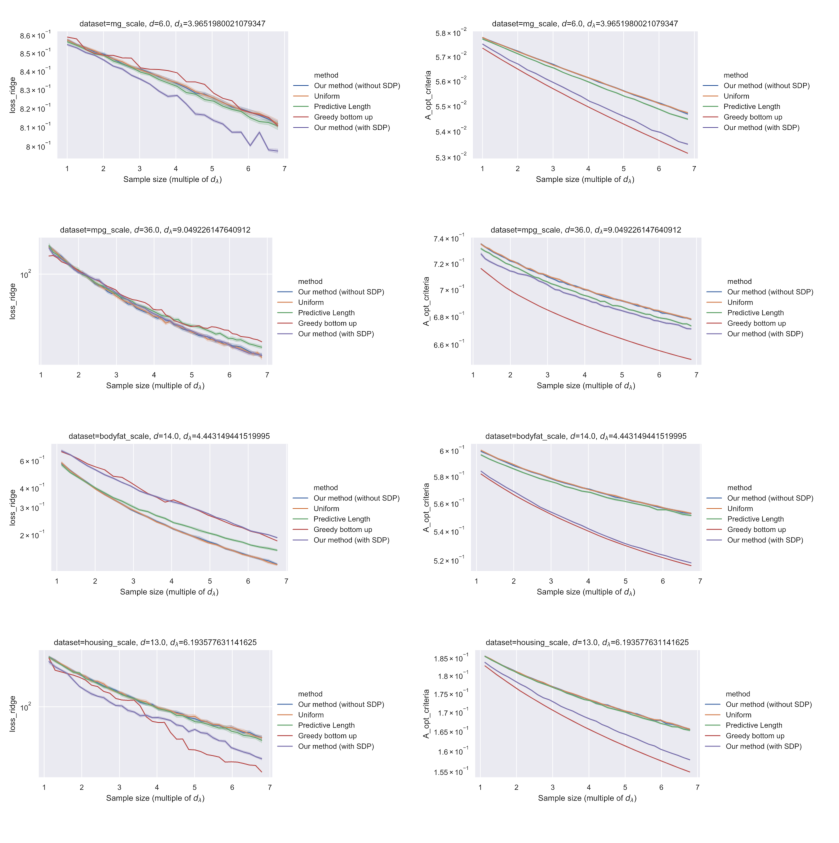
\includegraphics[width=\textwidth]{bayesian_figures/small_deff_ridge_and_a_opt.pdf}
    \caption{Ridge regression in low effective dimension on \texttt{libsvm} datasets.}
    \label{f:small_deff_ridge_and_a_opt}
\end{figure}


\section{Conclusions}

We proposed a new algorithm for finding
$(1+\epsilon)$-approximate Bayesian experimental designs by leveraging 
a fundamental connection with determinantal point processes. Compared
to the state-of-the-art approaches, our
method provides stronger theoretical guarantees in terms of the allowed
range of subset sizes, as well as
offering significantly better time complexity guarantees. At the same
time, our experiments show that on the task of A-optimal design the
proposed algorithm performs as well as or better than several methods that
are used in practice. 

\subsubsection*{Acknowledgements}

MWM would like to acknowledge ARO, DARPA, NSF and ONR for providing partial
  support of this work. Also, MWM and MD thank the NSF TRIPODS program
    and FL thanks the NPSC for funding.  The authors thank Uthaipon
  T.~Tantipongpipat for valuable discussions.


% \bibliographystyle{apalike}
% \bibliography{../pap}

% \newpage
% \appendix

% \onecolumn

\section{Properties of regularized DPPs}
\label{a:proofs}
In this section we provide proofs omitted from Sections \ref{s:r-dpp}
and \ref{s:guarantees}. We start with showing the fact that the
regularized DPP distribution $\DPPreg{p}(\X,\A)$ is a correlation DPP.
\begin{lemma}[restated Lemma \ref{l:correlation}]
  Given $\X$, $\A$, and $\D_p$ as in Theorem \ref{t:algorithm}, we have
  \begin{align*}
    \DPPreg{p}(\X,\A)= \DPPcor\big(\D_p +
    (\I-\D_p)^{\sfrac12}\,\D_p^{\sfrac12}\X(\A+\X^\top\D_p\X)^{-1}\X^\top\D_p^{\sfrac12}(\I-\D_p)^{\sfrac12}\big).
    \end{align*}
  \end{lemma}
  \begin{proof}
    First, we show this under the invertibility assumptions of Lemma
    \ref{t:reduction}, i.e., given that $\A$ and $\I-\D_p$ are
    invertible. In this case $\DPPreg{p}(\X,\A)=\DPPens(\L)$, where
    \begin{align}\L=\Dbt+
    \Dbt^{\sfrac12}\X\A^{-1}\X^\top
      \Dbt^{\sfrac12}\quad\text{ and }\quad\Dbt=\D_p(\I-\D_p)^{-1}.\label{eq:ensemble}
\end{align}
Converting this to
    a correlation kernel $\K$ and denoting $\Xt=\D_p^{\sfrac12}\X$, we obtain
    \begin{align*}
      \K&=\I-(\I+\L)^{-1}
\\      &=\I - \big(\I + (\I-\D_p)^{-1}\D_p +
(\I-\D_p)^{-\sfrac12}\Xt\A^{-1}\Xt^\top(\I-\D_p)^{-\sfrac12}\big)^{-1}
\\ &= \I - \big((\I-\D_p)^{-1} +
     (\I-\D_p)^{-\sfrac12}\Xt\A^{-1}\Xt^\top(\I-\D_p)^{-\sfrac12}\big)^{-1}
\\ &=\I -
     (\I-\D_p)^{\sfrac12}(\I+\Xt\A^{-1}\Xt^\top)^{-1}(\I-\D_p)^{\sfrac12}
      \\
      &\overset{(*)}{=}\I -
     (\I-\D_p)^{\sfrac12}\big(\I-\Xt\A^{-\sfrac12}
     (\I+\A^{-\sfrac12}\Xt^\top\Xt\A^{-\sfrac12})^{-1}
     \A^{-\sfrac12}\Xt^\top\big)(\I-\D_p)^{\sfrac12}
      \\
      &=\I - (\I-\D_p) +
     (\I-\D_p)^{\sfrac12}\Xt(\A+\Xt^\top\Xt)^{-1}\Xt^\top(\I-\D_p)^{\sfrac12}
\\ &=\D_p + (\I-\D_p)^{\sfrac12}\Xt(\A+\Xt^\top\Xt)^{-1}\Xt^\top(\I-\D_p)^{\sfrac12},
    \end{align*}
    where $(*)$ follows from Fact 2.16.19 in
    \cite{matrix-mathematics}. Note that converting from $\L$ to $\K$
    got rid of the inverses $\A^{-1}$  and $(\I-\D_p)^{-1}$ appearing
    in \eqref{eq:ensemble}. The intuition 
    is that when $\A$ or $\I-\D_p$ is non-invertible, then
    $\DPPreg{p}(\X,\A)$ is not an L-ensemble but it is still a
    correlation DPP. To show this, we use a limit argument. For
    $\epsilon\in[0,1]$, let $p_\epsilon=(1-\epsilon)p$ and
    $\A_\epsilon=\A+\epsilon\I$. Observe that if $\epsilon>0$ then $\A_\epsilon$ and
    $\I-\D_{p_{\epsilon}}$ are always invertible even if $\A$ and
    $\I-\D_p$ are not. Denote $\K_\epsilon$ as the
    above correlation kernel with $p$ replaced by $p_{\epsilon}$ and
    $\A$ replaced by $\A_{\epsilon}$. Note that all matrix operations
    defining kernel $\K_\epsilon$ are continuous w.r.t. $\epsilon\in[0,1]$, including the inverse, since
    $\A+\Xt^\top\Xt$ is assumed to be invertible. Therefore, the
    following equalities hold (with limits taken point-wise and $\epsilon>0$):
    \begin{align*}
      \DPPreg{p}(\X,\A) = \lim_{\epsilon\rightarrow
      0}\DPPreg{p_\epsilon}(\X,\A_{\epsilon}) =
      \lim_{\epsilon\rightarrow 0}\DPPcor(\K_\epsilon) = \DPPcor(\K),
    \end{align*}
where we did not have to assume invertibility of $\A$ or $\I-\D_p$.
\end{proof}
We now prove a lemma about combining a determinantal point process
with Bernoulli sampling, which itself is a DPP with a diagonal correlation
kernel.
\begin{lemma}[restated Lemma \ref{l:decomposition}]
  Let $\K$ and $\D$ be $n\times n$ psd matrices with eigenvalues between
0 and 1, and assume that $\D$ is diagonal. If\, $T\!\sim\DPPcor(\K)$ and
$R\sim\DPPcor(\D)$, then
\begin{align*}T\cup R\sim \DPPcor\big(\D+(\I-\D)^{\sfrac12}\K
  (\I-\D)^{\sfrac12}\big).
  \end{align*}
\end{lemma}
\begin{proof}
For this proof we will use the shorthand $\K_A$ for $\K_{A,A}$. If
$\D$ has no zeros on the diagonal then $\det(\D_A)>0$ for all
$A\subseteq[n]$ and
  \begin{align*}
    \Pr(A \subset T \cup R)
    &=\sum_{B\subset A}\Pr(R\cap A=A\setminus B) \ \Pr(B\subseteq T)\\
    &=\sum_{B\subset A}\det(\D_{A\setminus
      B})\det\!\big([\I-\D]_B\big)\,\det(\K_B) \\
    &=\sum_{B\subset A}\det(\D_{A\setminus
      B})\det\!\Big(\big[(\I-\D)^{\sfrac12}\K(\I-\D)^{\sfrac12}\big]_B\Big) \\
    &=\det(\D_A) \sum_{B\subset A}\det\!\Big(\big[\D^{-\sfrac12}
      (\I-\D)^{\sfrac12}\K(\I-\D)^{\sfrac12}\D^{-\sfrac12}\big]_{B}\Big)\\[-1mm]
    &\overset{(*)}{=}\det(\D_A)\det\!\Big(\I + \big[\D^{-\sfrac12}
      (\I-\D)^{\sfrac12}\K(\I-\D)^{\sfrac12}\D^{-\sfrac12}\big]_A\Big)\\
    &=\det\!\Big(\big[\D+ (\I-\D)^{\sfrac12}\K(\I-\D)^{\sfrac12}\big]_A\Big),
  \end{align*}
  where $(*)$ follows from a standard determinantal identity used to
  compute the L-ensemble partition function
  \cite[Theorem~2.1]{dpp-ml}. If $\D$ has zeros on the diagonal, a
  similar limit argument as in Lemma \ref{l:correlation} with
  $\D_\epsilon=\D+\epsilon\,\I$ holds.
\end{proof}
Next, we give a bound on the expected size of a regularized DPP.
\begin{lemma}[restated Lemma \ref{l:size}]
  Given any $\X\in\R^{n\times d}$, $p\in[0,1]^n$ and a psd matrix $\A$
  s.t.~$\sum_ip_i\x_i\x_i^\top\!+\A$ is
  full rank, let $S=T\cup \{i:b_i=1\}\sim \DPPreg{p}(\X,\A)$ be defined
as in Theorem \ref{t:algorithm}. Then
\begin{align*}
\E\big[|S|\big]\leq \E\big[|T|\big] + \E\Big[\sum_i b_i\Big] =
  d_{\A}\Big(\sum_ip_i\x_i\x_i^\top\Big) + \sum_i  p_i.
\end{align*}
\end{lemma}
\begin{proof}
For correlation kernels it is known that the expected size of $\DPPcor(\K)$
is $\tr(\K)$. Thus, using $\D_p=\diag(p)$, we can invoke Lemma \ref{l:correlation} to obtain
\begin{align*}
  \E\big[|S|\big]
  &= \tr\big(\D_p +
  (\I-\D_p)^{\sfrac12}\,\D_p^{\sfrac12}\X(\A+\X^\top\D_p\X)^{-1}
                    \X^\top\D_p^{\sfrac12}(\I-\D_p)^{\sfrac12}\big)
  \\ &\leq \tr(\D_p) +\tr\big(\D_p^{\sfrac12}
       \X(\A+\X^\top\D_p\X)^{-1}\X^\top\D_p^{\sfrac12}\big)
\\ &=\tr(\D_p) +\tr\big(\X^\top\D_p\X (\A+\X^\top\D_p\X)^{-1}\big) =
     \tr(\D_p) + d_{\A}(\X^\top\D_p\X),
\end{align*}
from which the claim follows.
\end{proof}
Next, we show two expectation inequalities for the matrix inverse and
matrix determinant.
\begin{lemma}[restated Lemma \ref{t:expectations}]
Whenever $S\sim \DPPreg{p}(\X,\A)$ is a well-defined distribution it holds that
\begin{align}
  \E\Big[\big(\X_S^\top\X_S+\A\big)^{-1}\Big]
  &\preceq \Big(
    \sum_ip_i\x_i\x_i^\top +\A \Big)^{-1},\label{eq:sqinv2}
  \\
\E\Big[\det\!\big(\X_S^\top\X_S+\A\big)^{-1}\Big]
  &\leq\det\!\Big(
    \sum_ip_i\x_i\x_i^\top +\A \Big)^{-1}.\label{eq:det2}
\end{align}
\end{lemma}
\begin{proof}
For a square matrix $\M$, define its adjugate, denoted $\adj(\M)$, as a matrix
whose $i,j$-th entry is $(-1)^{i+j}\det(\M_{-j,-i})$, where
$\M_{-j,-i}$ is the matrix $\M$ without $j$th row and $i$th column. If
$\M$ is invertible, then $\adj(\M) = \det(\M)\M^{-1}$. Now, let
$b_i\sim\mathrm{Bernoulli}(p_i)$ be independent random variables. As seen
in previous section, the identity
$\E[\det(\sum_ib_i\x_i\x_i^\top+\A)]=\det(\sum_ip_i\x_i\x_i^\top+\A)$ gives
us the normalization constant for $\DPPreg{p}(\X,\A)$. Moreover, as
noted in a different context by \cite{determinantal-averaging}, when
applied entrywise to the adjugate matrix, this identity implies that
$\E[\adj(\sum_ib_i\x_i\x_i^\top+\A)]=\adj(\sum_ip_i\x_i\x_i^\top+\A)$. Let
$\Ic$ denote the set of all subsets $S\subseteq [n]$ such that
$\X_S^\top\X_S+\A$ is invertible. We have
\begin{align*}
  \E\Big[\big(\X_S^\top\X_S+\A\big)^{-1}\Big]
  &= \sum_{S\in\Ic}\big(\X_S^\top\X_S+\A\big)^{-1}
\frac{\det(\X_S^\top\X_S+\A)}{\det(\sum_ip_i\x_i\x_i^\top+\A)}\ \prod_{i\in
    S}p_i\prod_{i\not\in S}(1-p_i)
\\ &=\sum_{S\in\Ic}\frac{\adj(\X_S^\top\X_S+\A\big)}
{\det(\sum_ip_i\x_i\x_i^\top+\A)}\ \prod_{i\in
     S}p_i\prod_{i\not\in S}(1-p_i)
\\ &\preceq \sum_{S\subseteq[n]}\frac{\adj(\X_S^\top\X_S+\A\big)}
{\det(\sum_ip_i\x_i\x_i^\top+\A)}\ \prod_{i\in
     S}p_i\prod_{i\not\in S}(1-p_i)
\\ &=\frac{\E\big[\!\adj(\sum_i
     b_i\x_i\x_i^\top+\A)\big]}{\det(\sum_ip_i\x_i\x_i^\top+\A)}
  \\
  &=\frac{\adj(\sum_ip_i\x_i\x_i^\top+\A)}{\det(\sum_ip_i\x_i\x_i^\top+\A)}
    = \Big(\sum_ip_i\x_i\x_i^\top+\A\Big)^{-1}.
\end{align*}
Note that if $\Ic$ contains all subsets of $[n]$, for example when
$\A\succ\zero$, then the inequality turns into equality. Thus, we
showed \eqref{eq:sqinv2}, and \eqref{eq:det2} follows even more easily:
\begin{align*}
  \E\Big[\!\det\!\big(\X_S^\top\X_S+\A\big)^{-1}\Big]
  &= \sum_{S\in\Ic}
\frac{1}{\det(\sum_ip_i\x_i\x_i^\top+\A)}\ \prod_{i\in
    S}p_i\prod_{i\not\in S}(1-p_i)
\leq \det\!\Big(\sum_i p_i\x_i\x_i^\top\Big)^{\!-1}\!,
\end{align*}
where the equality holds if $\Ic$ consists of all subsets of $[n]$.
\end{proof}

\section{Comparison of different effective dimensions}
\label{a:deff}
In this section we compare the two notions of effective dimension for
Bayesian experimental design considered in this work. Here, we let
$\X$ be the full $n\times d$ design matrix and use $k$ to denote the
desired subset size. Recall that the effective dimension is  defined
as a function of the data covariance matrix $\Sigmab_\X=\X^\top\X$ and
the prior precision matrix $\A$:
It is given by $d_{\A} =
\tr\big(\Sigmab_\X(\A+\Sigmab_\X)^{-1}\big)$. In
\cite{regularized-volume-sampling} it was suggested that $d_{\A}$
should also be used as the effective dimension for the experimental
design problem. Theorem \ref{t:q1} suggests it may not reflect the true degrees
of freedom of the problem because it does not scale with subset size
$k$. Instead we propose to use the \emph{scaled effective dimension}
$d_{\frac nk\!\A}$. Thus, the two definitions we are comparing can be
summarized as follows:
\begin{description}
  \item[Full effective dimension]\quad\ \ \,$d_{\A} =
    \tr\big(\Sigmab_\X(\A+\Sigmab_\X)^{-1}\big)$,
    \item[Scaled effective dimension] $d_{\frac nk\!\A} =
      \tr\big(\Sigmab_\X(\tfrac nk\A + \Sigmab_\X)^{-1}\big)$.
    \end{description}
    Here, we demonstrate that these two effective dimensions can be
    very different for some matrices and quite similar on others. For
    simplicity, we consider two diagonal data covariance matrices as
    our examples: \emph{identity covariance}, $\Sigmab_1 = \I$, and an
    \emph{approximately low-rank covariance}, $\Sigmab_2 =
    (1-\epsilon)\frac ds \I_S+\epsilon\I$, where $\I_S$ is the
    diagonal matrix with ones on the entries indexed by subset
    $S\subseteq [d]$ of
    size $s<d$ and zeros
    everywhere else. The second matrix is scaled in such way so that
    $\tr(\Sigmab_1)=\tr(\Sigmab_2)$. We use $d=100$, $s=10$ and
    $\epsilon=10^{-2}$. The prior precision matrix is
    $\A=10^{-2}\,\I$. Figure \ref{f:deff} plots the scaled effective
    dimension $d_{\frac nk\!\A}$ as a function of $k$, against the
    full effective dimension for both examples. Unsurprisingly, for
    the identity covariance the full effective dimension is almost
    $d$, and the scaled effective dimension goes up very quickly to
    match it. On the other hand, for the approximately low-rank
    covariance, $d_{\A}\approx 55$ is considerably less then
    $d=100$. Interestingly, the gap between the $d_{\frac nk\!\A}$ and 
    $d_{\A}$ for moderately small values of $k$ is even bigger. Our
    theory suggests that $d_{\frac nk\!\A}$ is a valid indicator of
    Bayesian degrees of freedom when $k\geq C\cdot d_{\frac nk\!\A}$
    for some small constant $C$ (Theorem \ref{t:q1} has $C=4$, but we
    believe this can be improved to $1$). While for the identity
    covariance the condition $k\geq
    d_{\frac nk\!\A}$ is almost equivalent to $k\geq d_{\A}$, in the
    approximately low-rank case, $k\geq d_{\frac nk\!\A}$ holds for
    $k$ as small as 20, much less than $d_{\A}$.
    \begin{figure}[htbp]
      \centering
      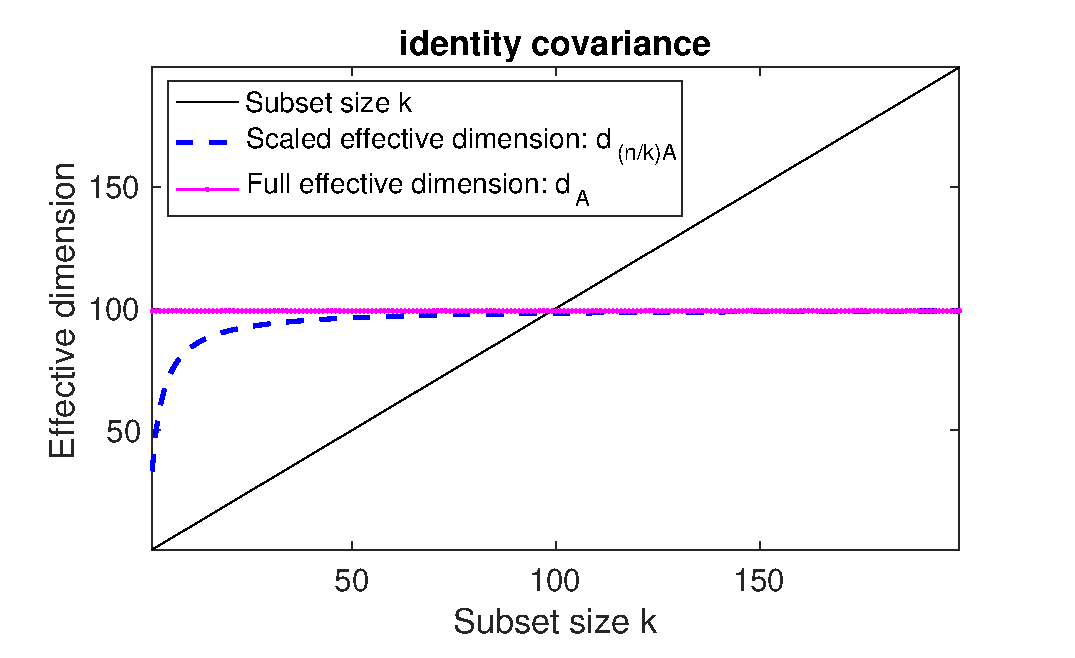
\includegraphics[width=0.5\textwidth]{../figs/deff_identity}\nobreak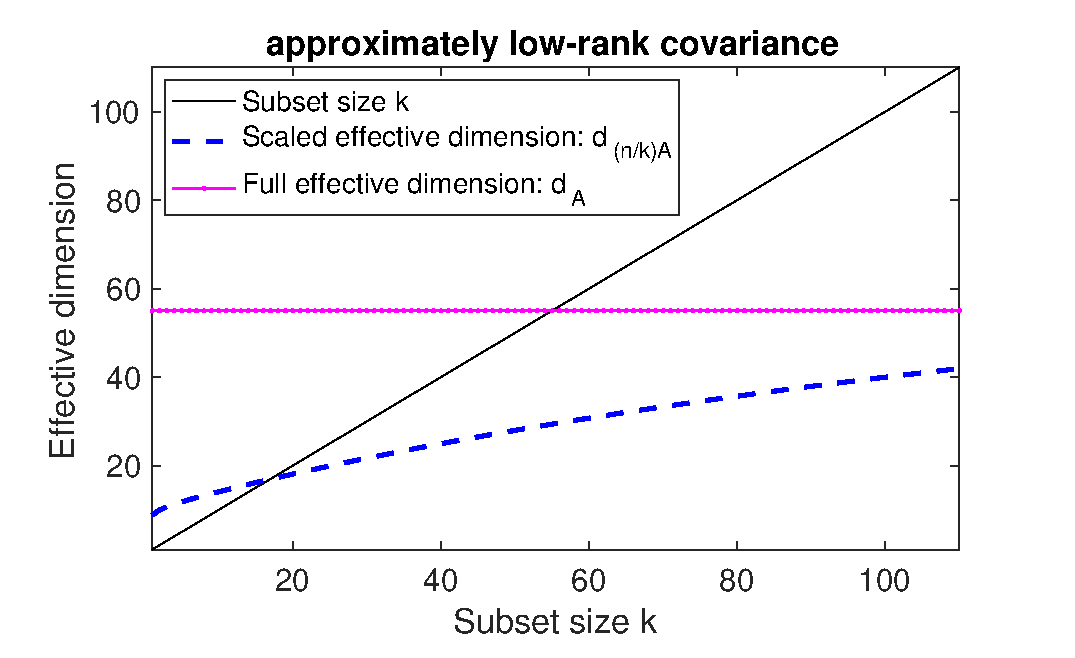
\includegraphics[width=0.5\textwidth]{../figs/deff_lowrank}
      \caption{Scaled effective dimension compared to the full effective
        dimension for two diagonal data covariance matrices, with
      $\A=10^{-2}\,\I$.}
      \label{f:deff}
    \end{figure}

\section{Additional details for the experiments}
\label{a:experiments}
\section*{Additional Experiments}

This section presents additional details and experimental results omitted from
the main body of the paper. In addition to the \texttt{mg\_scale} dataset presented in
Section~\ref{s:experiments}, we also benchmarked on three other data sets
described in Table~\ref{tab:libsvm-datasets}.
\begin{table}[ht]
    \centering
    \caption{\cite{libsvm} datasets used in experiments}
    \label{tab:libsvm-datasets}
    \begin{tabular}[t]{lcccc}
        \toprule
        & \texttt{mg\_scale} & \texttt{bodyfat\_scale} & \texttt{mpg\_scale} & \texttt{housing\_scale} \\
        \midrule
        $n$ & 1385 & 252 & 392 & 506 \\
        $d$ & 6 & 14 & 7 & 13\\
        \bottomrule
    \end{tabular}
\end{table}

The A-optimality values obtained are illustrated in Figure~\ref{f:obj-grid}.
The general trend observed in Section~\ref{s:experiments} of our method
(without SDP) outperforming independent sampling methods (uniform and
predictive length) and our method (with SDP) matching the performance of the
greedy bottom up method continues to hold across the additional datasets considered.

\begin{figure}[htpb]
    \centering
    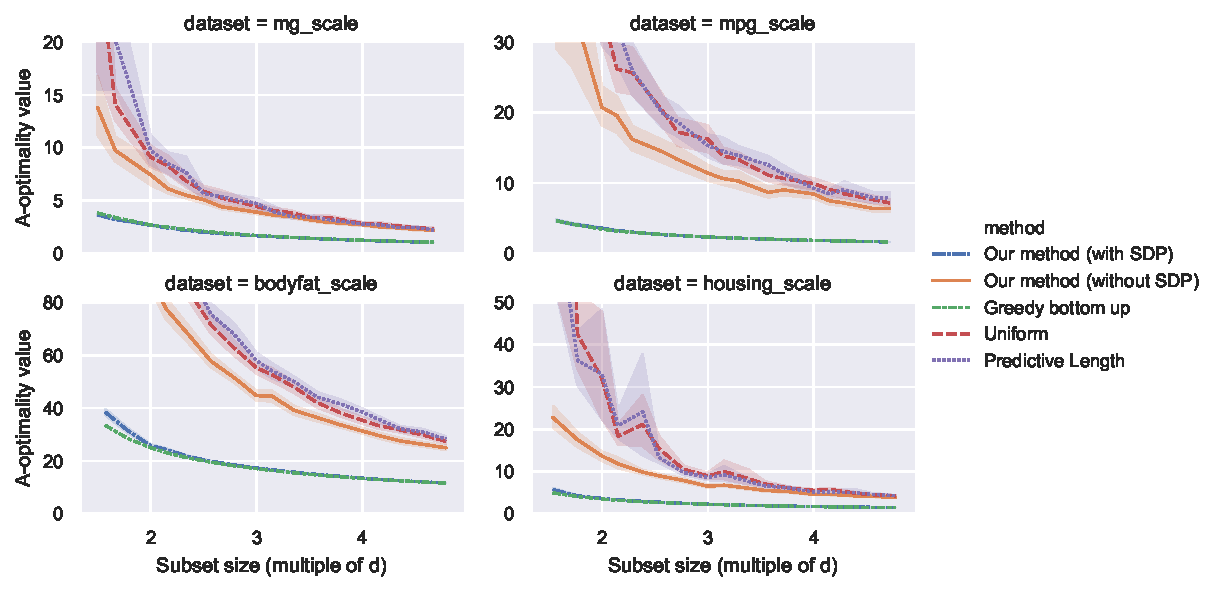
\includegraphics[width=\textwidth]{bayesian_figures/obj_grid.pdf}
    \caption{A-optimality values achieved by the methods compared. In all cases
        considered, we found our method (without SDP) to be superior to independent
        sampling methods like uniform and predictive length sampling. After paying the price
        to solve an SDP, our method (with SDP) is able to consistently match the performance
        of a greedy method which has been noted
        \cite{chamon2017approximate} to work well empirically.}
    \label{f:obj-grid}
\end{figure}

The relative ranking and overall order of magnitude differences
between runtimes (Figure~\ref{f:runtimes}) are also similar across the various
datasets. An exception to the rule is on $\texttt{mg\_scale}$, where we see
that our method (without SDP) costs more than the greedy method
(whereas everywhere else it costs~less).

\begin{figure}[htpb]
    \centering
    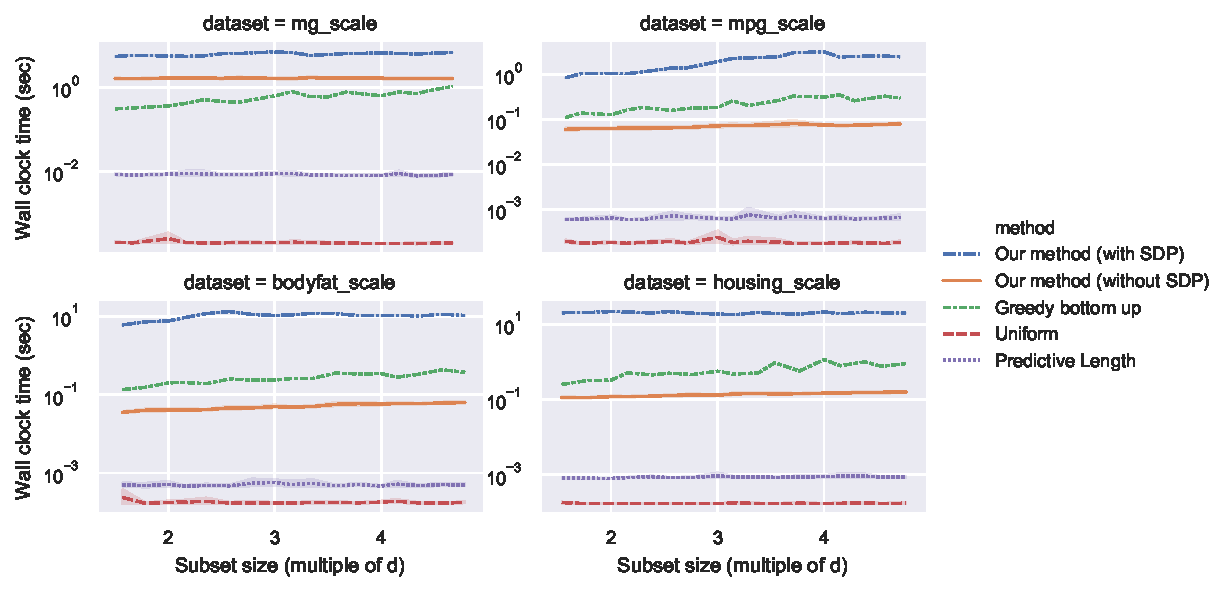
\includegraphics[width=\textwidth]{bayesian_figures/runtime_grid.pdf}
    \caption{Runtimes of the methods compared. Our method (without SDP) is
        within an order of magnitude of greedy bottom up and faster in 3 out of
        4 cases. The gap between our method with and without SDP is
        attributable to the SDP solver, making investigation of more efficient
        solvers and approximate solutions an interesting direction for future
        work.
    }
    \label{f:runtimes}
\end{figure}

The claim that $f_{\A}(\frac{k}{n} \Sigmab_\X)$ is an appropriate
quantity to summarize the contribution of problem-dependent factors
on the performance of Bayesian A-optimal designs is further evidenced in Figure~\ref{f:ratios}.
Here, we see that after normalizing the A-optimality values by this
quantity, the remaining quantities are all on the same scale and close to $1$.

\begin{figure}[htpb]
    \centering
    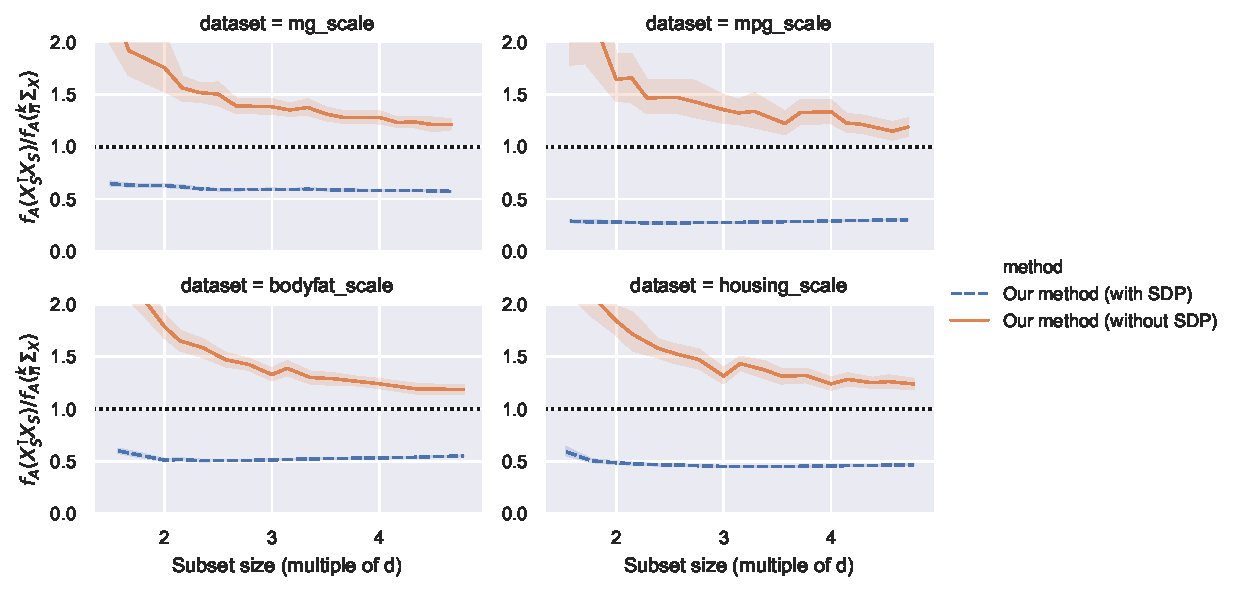
\includegraphics[width=\textwidth]{bayesian_figures/ratios_grid.pdf}
    \caption{The ratio controlled by Lemma~\ref{l:guarantees}. This ratio converges
        to $1$ as $k \to n$ and is close to $1$ across all
        real world datasets,
        suggesting that $f_{\A}(\frac{k}{n} \Sigmab_\X)$
        is an appropriate problem-dependent scale for Bayesian A-optimal
        experimental design.
    }
    \label{f:ratios}
\end{figure}

% The choice of $\lambda=43$ is motivated by keeping 95\% of the spectral
% mass. Figure~\ref{fig:scree} shows a scree plot for \texttt{mpg\_scale}
% after applying a polynomial kernel, where we see that the majority
% of the spectral mass is contained in the top few eigenvalues.

% \begin{figure}[htbp]
%     \centering
%     % \hspace{-0.55cm}
%     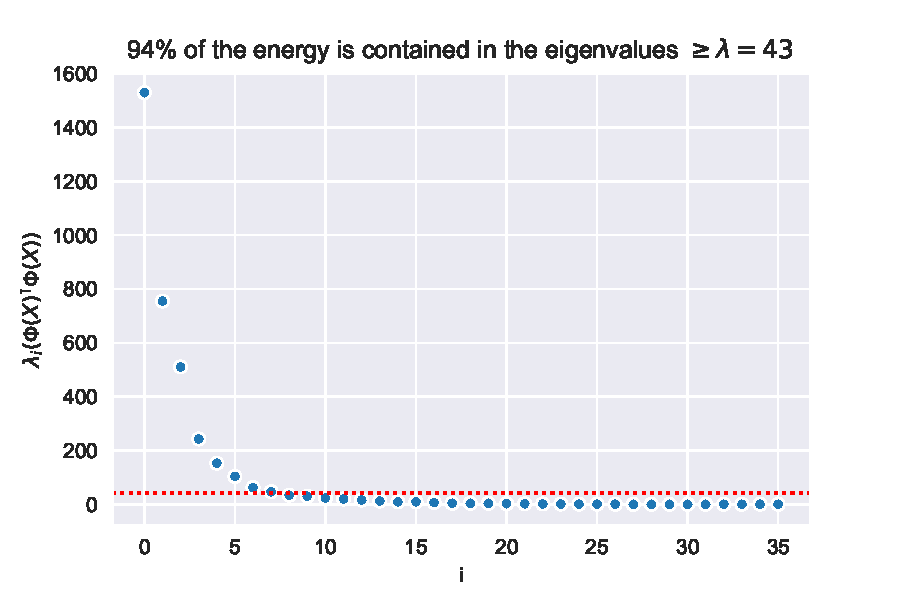
\includegraphics[width=0.5\textwidth]{Figures/screeplot.pdf}
%     \caption{
%         To determine the amount of regularization $\lambda$, a scree
%         plot of the eigenvalues of the polynomially expanded
%         covariance matrix $\Phi(X)^\top \Phi(X)$.
%     }
%     \label{fig:scree}
% \end{figure}

In addition to \texttt{mg\_scale}, the results for the low effective dimension
($d_\lambda$) ridge regression experiments on the remaining \texttt{libsvm}
datasets are shown in Figure~\ref{f:small_deff_ridge_and_a_opt}.

\begin{figure}[htpb]
    \centering
    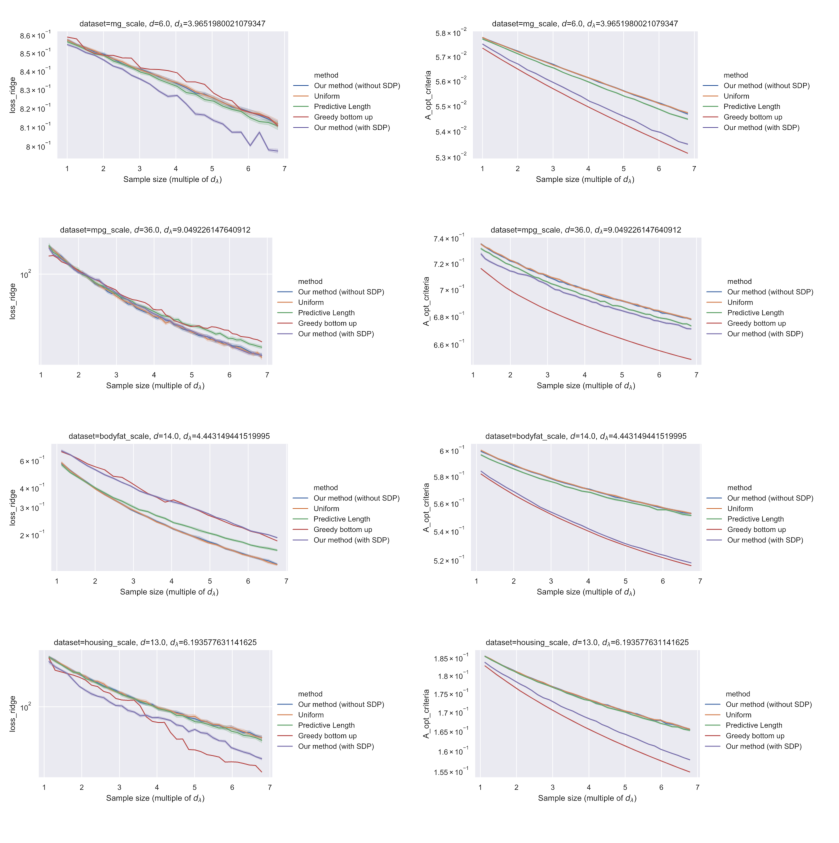
\includegraphics[width=\textwidth]{bayesian_figures/small_deff_ridge_and_a_opt.pdf}
    \caption{Ridge regression in low effective dimension on \texttt{libsvm} datasets.}
    \label{f:small_deff_ridge_and_a_opt}
\end{figure}


\end{document}
